\documentclass[aspectratio=169,11pt]{beamer}
\usepackage{teaching_slides}
\usetikzlibrary{positioning,calc}

% Figures are reused from the PhD decks (Fall/L9, Fall/L10); news clippings live in ./resources.
\graphicspath{{./resources/}{../Fall/L9 - Quasi Experiments/}{../Fall/L9 - Quasi Experiments/resources/}{../Fall/L10 - More Quasi Experiments/resources/}}

\tikzset{dag/.style={draw, circle, minimum size=9mm, inner sep=1pt}}

\title{Empirical Methods for Thesis Writers}
\subtitle{Causal Inference and Research Design}
\author{Chris Conlon \\ NYU Stern}
\date{Fall 2026}

% Rewritten Nov 2026 from the Sep 2024 thesis-writers deck (source lost; text recovered
% from Dropbox/undergrad_lecture/undergrad_lecture.pdf) and the Fall 2026 PhD decks
% L7 (causal diagrams), L8 (IV/LATE), L9 (event studies, DiD), L10 (synth, RD, staggered DiD).

\begin{document}
\maketitle

% =====================================================================
\section{How Not to Do Empirical Research}
% =====================================================================

\begin{frame}{How not to do empirical research}
\begin{columns}[c]
\begin{column}{0.48\textwidth}
\centering
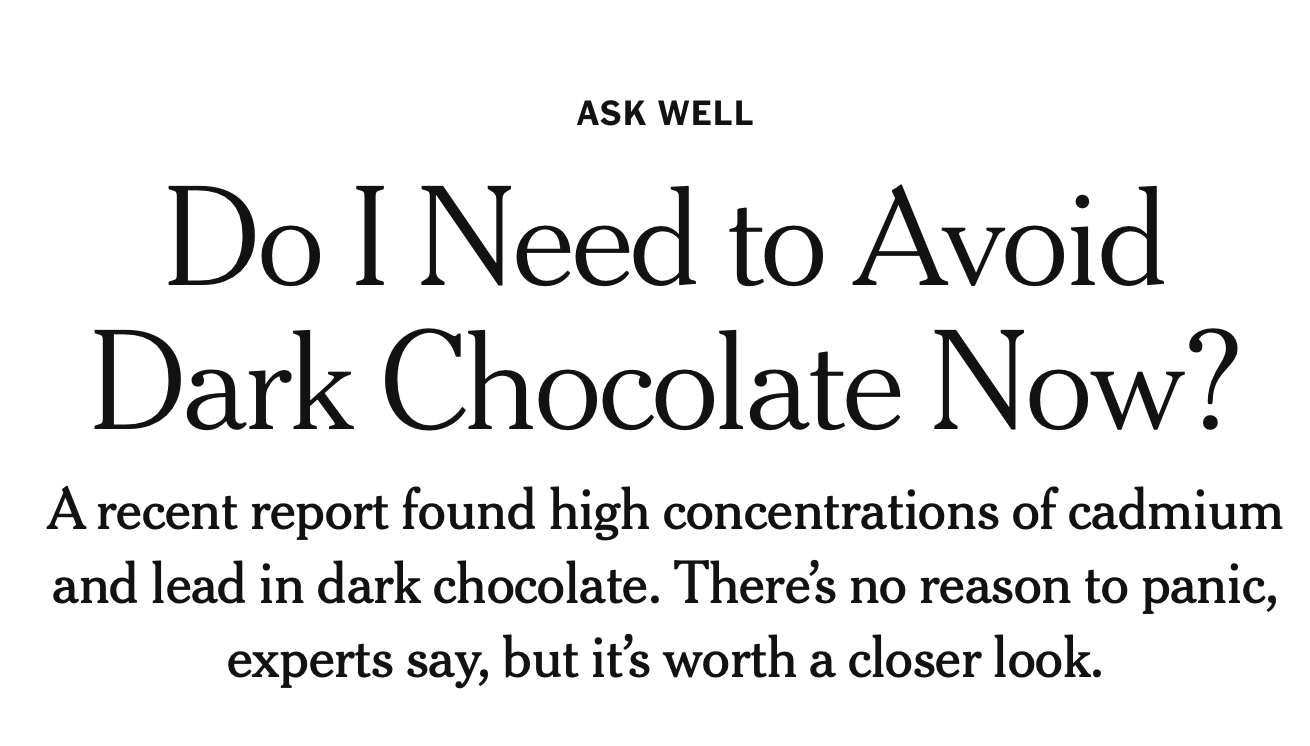
\includegraphics[width=0.85\textwidth]{news_avoid_chocolate.png}\\[0.6em]
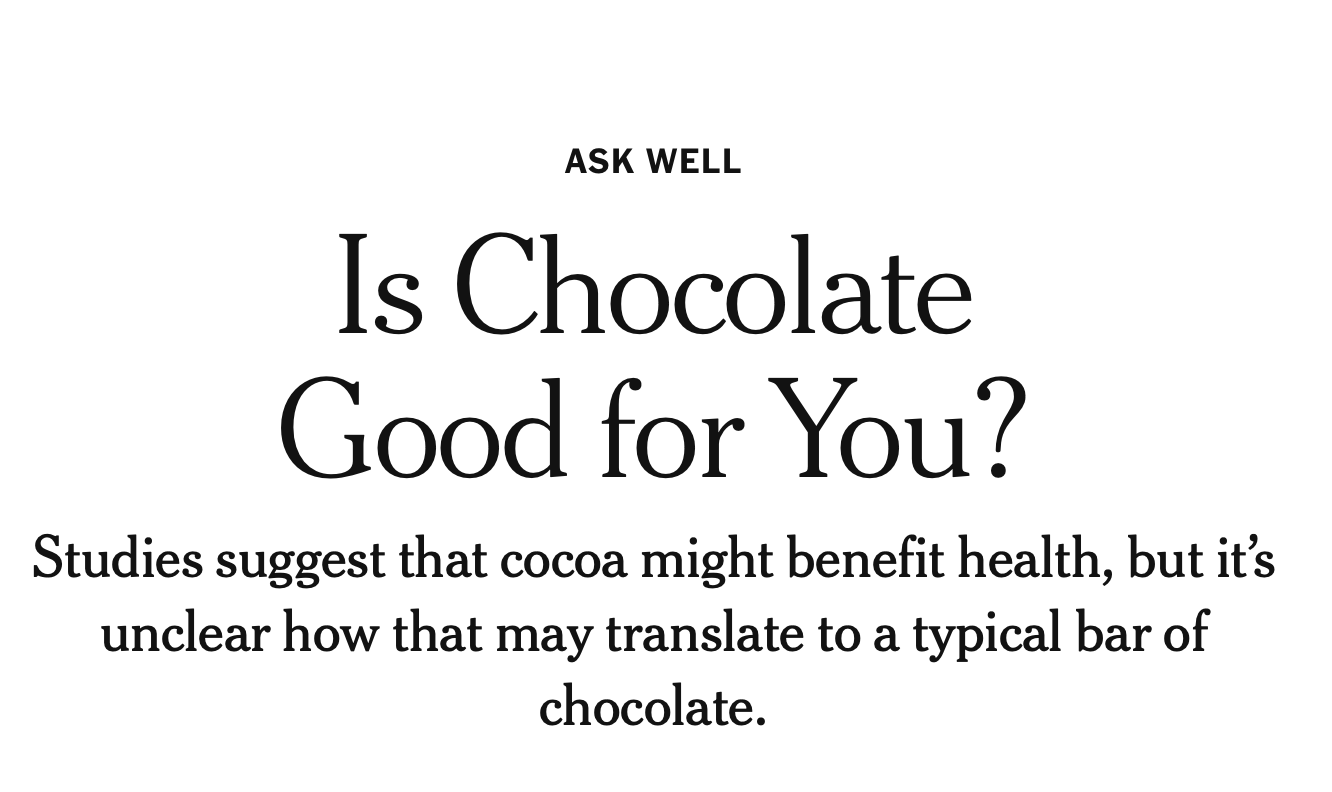
\includegraphics[width=0.85\textwidth]{news_chocolate_good.png}
\end{column}
\begin{column}{0.48\textwidth}
\centering
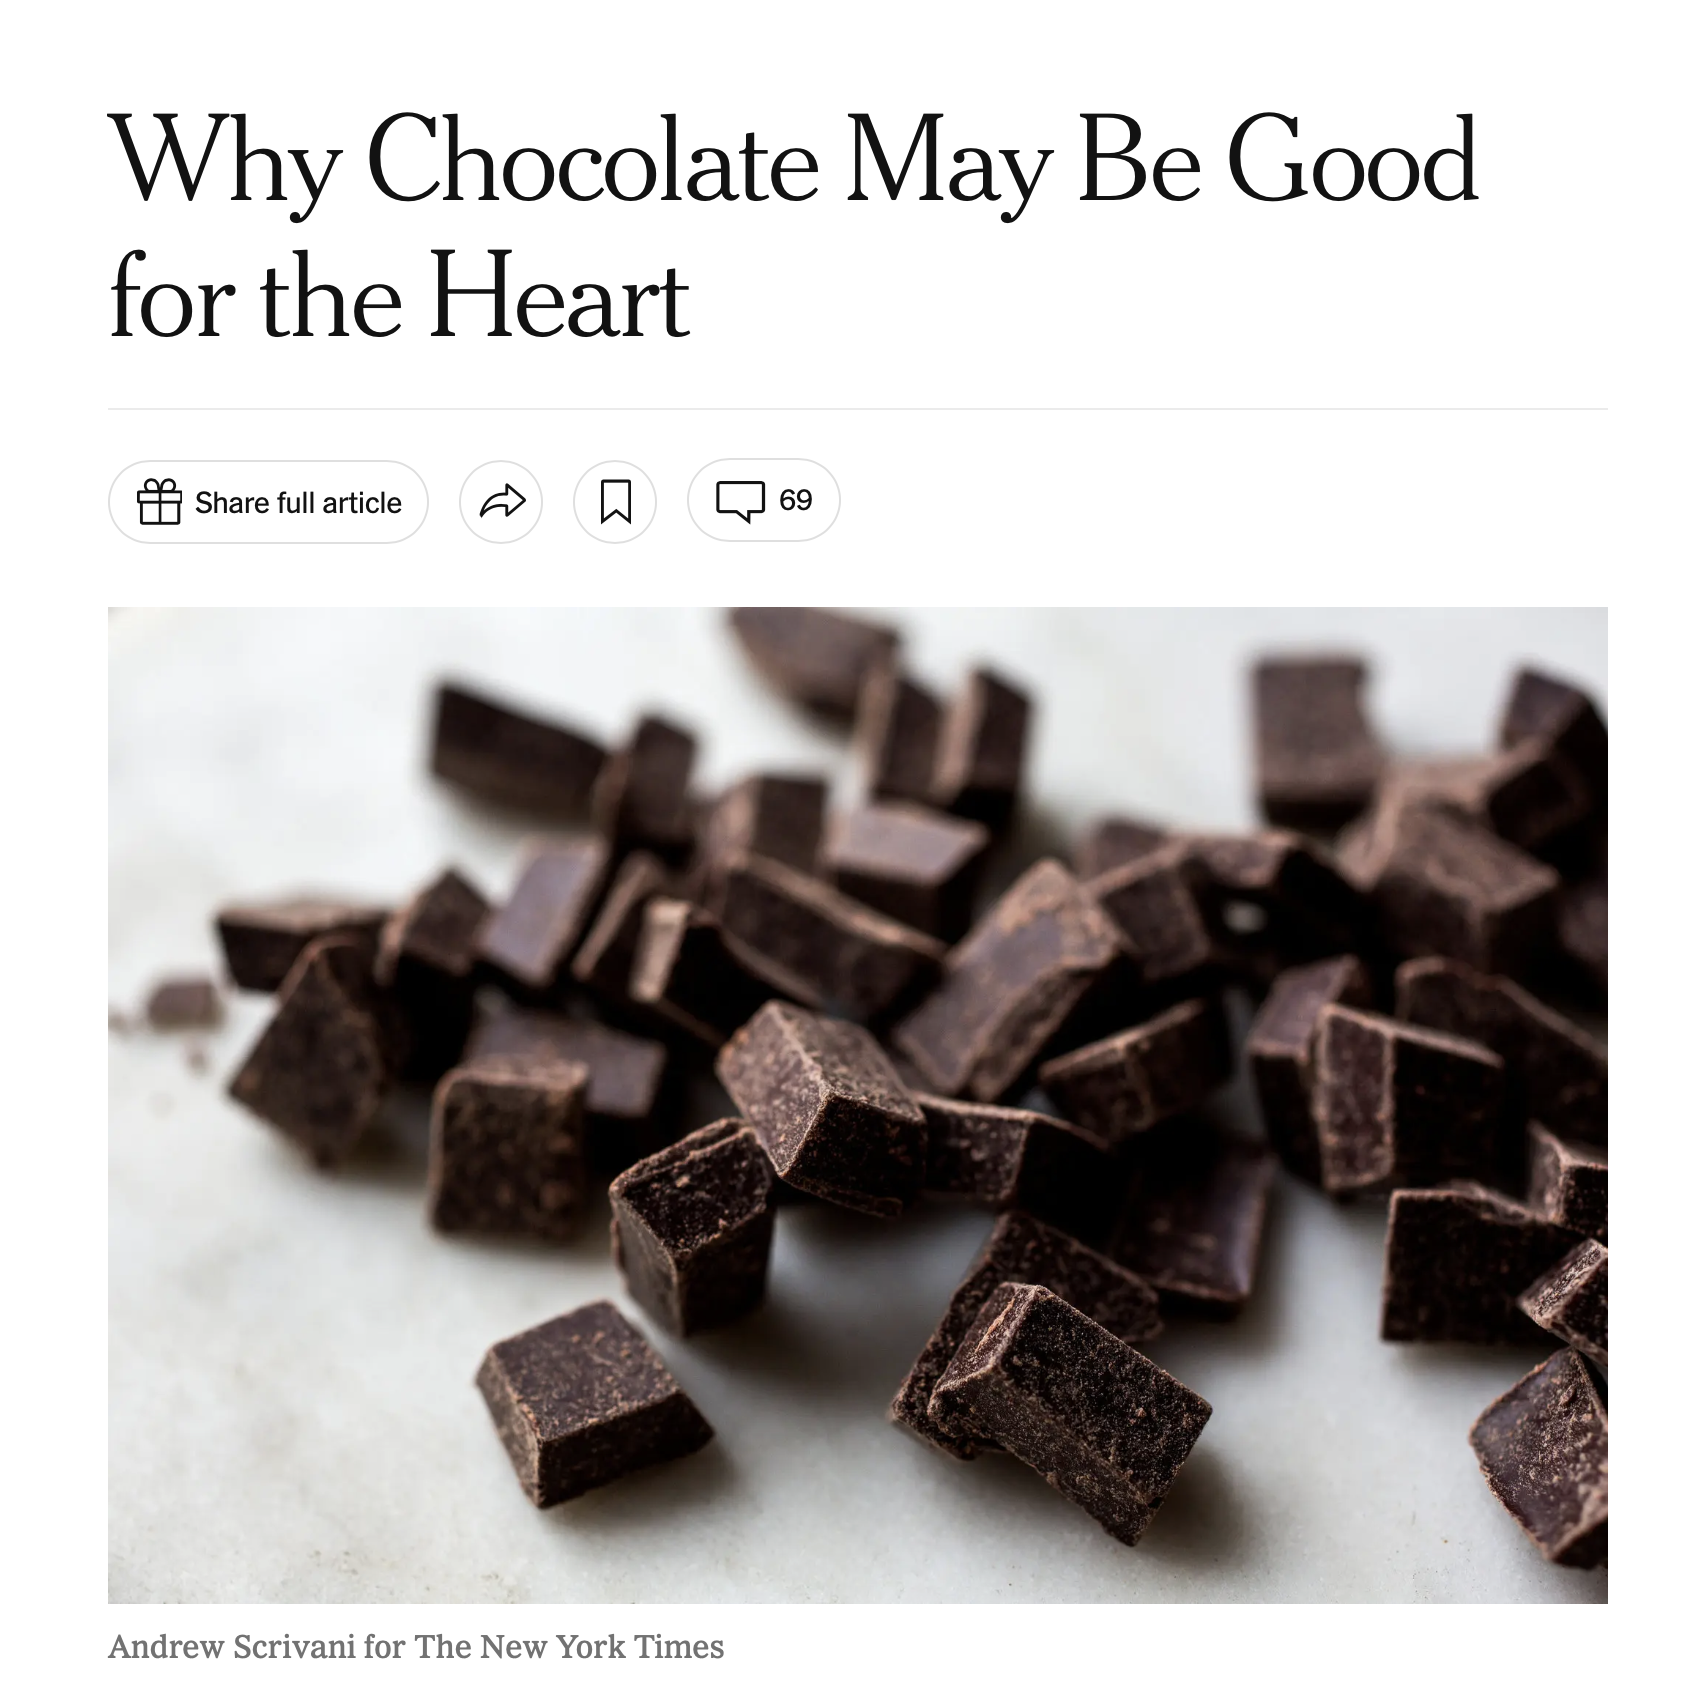
\includegraphics[width=\textwidth]{news_chocolate_heart.png}
\end{column}
\end{columns}
\end{frame}


\begin{frame}{How not to do empirical research (continued)}
\begin{columns}[c]
\begin{column}{0.5\textwidth}
\centering
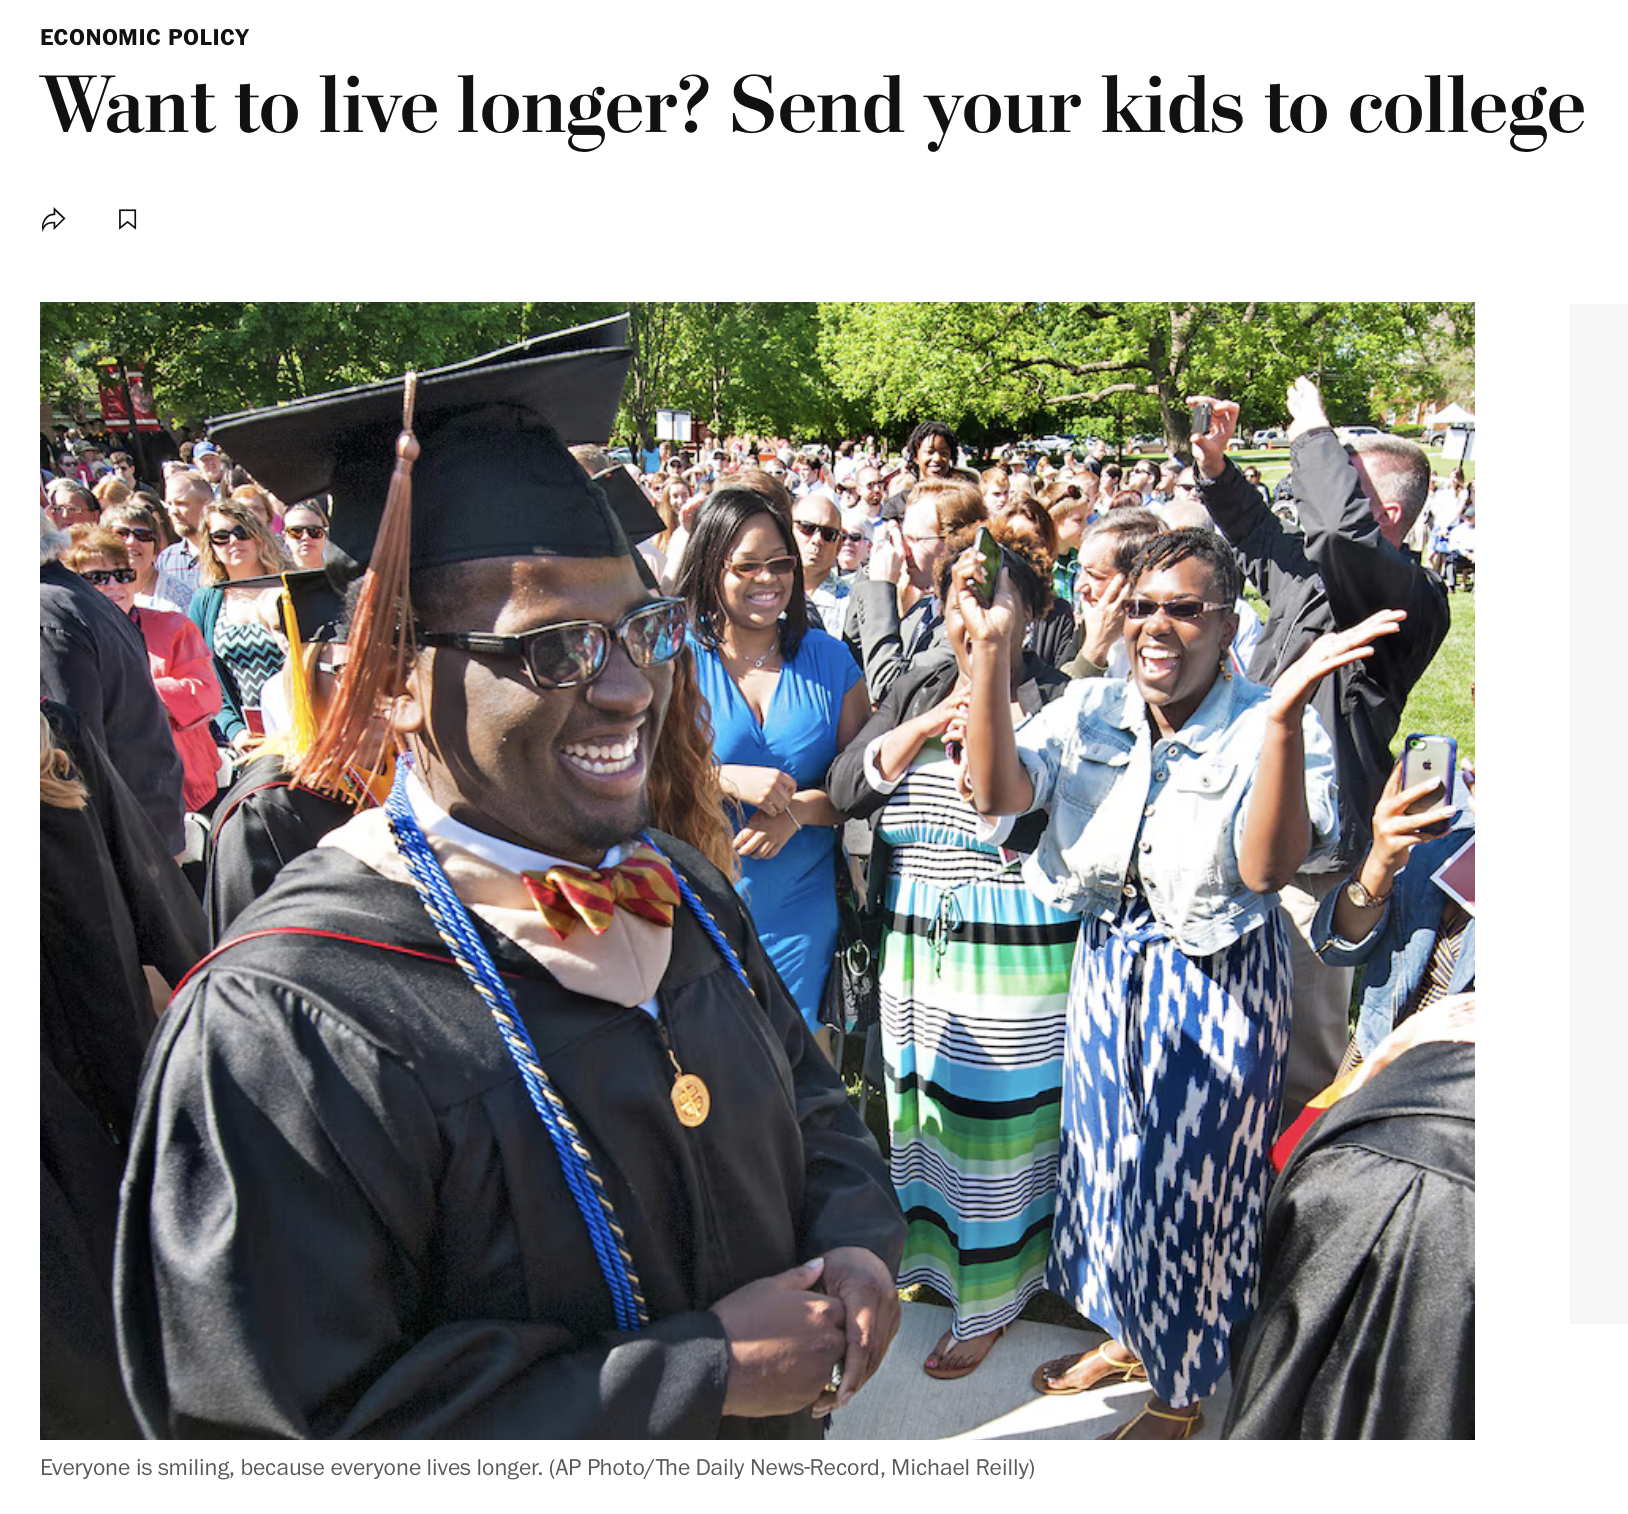
\includegraphics[width=\textwidth]{news_college_longevity.png}
\end{column}
\begin{column}{0.48\textwidth}
Parents of college graduates live longer.
\begin{itemize}
	\item What is the \alert{mechanism}?
	\item What else differs between families whose kids go to college and families whose kids don't?
	\item If you could run an \alert{experiment} to test this, what would it look like?
\end{itemize}
\medskip
Hold on to that last question. It is the most useful habit in this lecture.
\end{column}
\end{columns}
\end{frame}


\begin{frame}{What would Tolstoy say?}
\begin{center}
\emph{All good empirical papers are alike; each flawed paper is flawed in its own way.}
\end{center}
\bigskip
A good empirical paper has
\begin{itemize}
	\item A clear \alert{research question}
	\item A plausible \alert{mechanism}
	\item A well-defined \alert{counterfactual}: what would have happened otherwise?
\end{itemize}
\bigskip
Running example for today: \alert{what is the effect of writing a senior thesis at Stern on your lifetime earnings?}
\begin{itemize}
	\item What are the mechanisms? What is the counterfactual?
\end{itemize}
\end{frame}


\begin{frame}{Plan for today}
\begin{enumerate}
	\item \alert{The counterfactual}: what a causal effect is, and why comparing groups usually fails
	\item \alert{What to control for}: drawing your assumptions as pictures
	\item \alert{Where counterfactuals come from}: a map of research designs
	\begin{itemize}
		\item Lotteries and natural experiments (instrumental variables)
		\item Before and after: event studies and difference-in-differences
		\item One treated unit: synthetic control
		\item Cutoffs: regression discontinuity
	\end{itemize}
	\item \alert{A checklist for your thesis}
\end{enumerate}
\bigskip
Goal: you leave knowing \emph{which questions to ask}. The formulas are easy to look up later.
\end{frame}


% =====================================================================
\section{The Counterfactual}
% =====================================================================

\begin{frame}{Defining the counterfactual}
Each student $i$ has two \alert{potential outcomes}:
\begin{itemize}
	\item $Y_i(1)$: lifetime earnings if $i$ writes a thesis
	\item $Y_i(0)$: lifetime earnings if $i$ does not
\end{itemize}
The \alert{causal effect} for student $i$ is $Y_i(1) - Y_i(0)$.
\medskip

\alert{The fundamental problem of causal inference:} we see each student in only one world.
\begin{center}\small
\begin{tabular}{lccc}
\toprule
Student & $Y_i(1)$ & $Y_i(0)$ & Wrote thesis? \\
\midrule
Ana & \$4.1M & \alert{?} & Yes \\
Ben & \alert{?} & \$3.2M & No \\
Cal & \$3.6M & \alert{?} & Yes \\
\bottomrule
\end{tabular}
\end{center}
Every method today is a way of filling in the \alert{?}s with someone or something else.
\end{frame}


\begin{frame}{The naive comparison}
Compare average earnings of thesis writers to non-writers:
\begin{align*}
\underbrace{\E[Y \mid \text{thesis}] - \E[Y \mid \text{no thesis}]}_{\text{what we see}}
= \underbrace{\text{effect of the thesis}}_{\text{what we want}}
+ \underbrace{\E[Y(0) \mid \text{thesis}] - \E[Y(0) \mid \text{no thesis}]}_{\text{\alert{selection bias}}}
\end{align*}
\begin{itemize}
	\item Selection bias: would thesis writers have earned more \alert{even without the thesis}?
	\item Almost certainly yes: higher GPA, more ambition, better recommendations, more interest in research.
	\item Same problem as chocolate and longevity. The groups were different \alert{before} the ``treatment.''
\end{itemize}
\end{frame}


\begin{frame}{Why experiments work}
Suppose we \alert{flipped a coin} to decide who writes a thesis.
\begin{itemize}
	\item Then the two groups are the same on average, in everything: GPA, ambition, family background, things we can't measure.
	\item Selection bias is zero, and the simple comparison of means \alert{is} the causal effect.
\end{itemize}
\bigskip
We usually can't flip the coin. So the rest of this lecture is about finding situations that are
\begin{center}
\alert{as good as random}
\end{center}
and being honest about what has to be true for that to hold.
\end{frame}


\begin{frame}{Effect for whom?}
``The effect'' is not one number. Be clear about \emph{whose} effect you estimate:
\begin{itemize}
	\item \alert{Average effect (ATE)}: if we made a random Stern student write a thesis.
	\item \alert{Effect on the treated (ATT)}: for the students who actually chose to write one.
	\item \alert{Local effect (LATE)}: for students whose choice was changed by your source of variation (more on this soon).
\end{itemize}
\medskip
These can differ a lot when people \alert{choose} treatment because they expect to benefit.
\medskip
\begin{itemize}
	\item Your thesis should say which one you estimate, and whether it speaks to the policy question you care about (\alert{external validity}).
\end{itemize}
\end{frame}


% =====================================================================
\section{What Should I Control For?}
% =====================================================================

\begin{frame}{Drawing your assumptions}
\begin{columns}
\begin{column}{0.42\textwidth}
\begin{center}
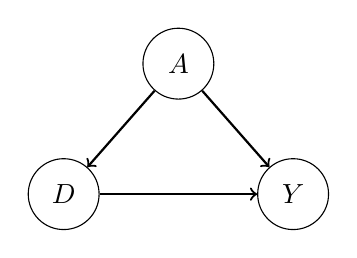
\begin{tikzpicture}[node distance=20mm]
	\node[dag] (D) {$D$};
	\node[dag, right=of D] (Y) {$Y$};
	\node[dag, above=12mm of $(D)!0.5!(Y)$] (A) {$A$};
	\draw[->, thick] (D) -- (Y);
	\draw[->, thick] (A) -- (D);
	\draw[->, thick] (A) -- (Y);
\end{tikzpicture}
\end{center}
\smallskip
{\small $D$ = thesis, $Y$ = earnings, $A$ = ability / ambition}
\end{column}
\begin{column}{0.56\textwidth}
\begin{itemize}
	\item A \alert{causal diagram} (DAG): arrows are causal effects.
	\item Two routes connect $D$ and $Y$:
	\begin{itemize}
		\item $D \rightarrow Y$: the \alert{causal path} we want
		\item $D \leftarrow A \rightarrow Y$: a \alert{backdoor path}, which creates correlation even if the thesis does nothing
	\end{itemize}
	\item Every \alert{missing} arrow is an assumption. Drawing the picture forces you to state them.
	\item Your research design is a plan to \alert{block every backdoor path}.
\end{itemize}
\end{column}
\end{columns}
\end{frame}


\begin{frame}{Good controls: blocking a backdoor}
\begin{columns}
\begin{column}{0.42\textwidth}
\begin{center}
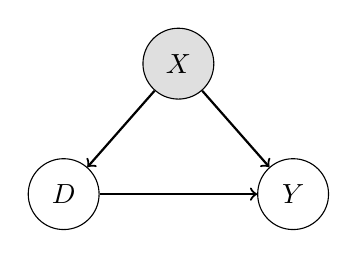
\begin{tikzpicture}[node distance=20mm]
	\node[dag] (D) {$D$};
	\node[dag, right=of D] (Y) {$Y$};
	\node[dag, above=12mm of $(D)!0.5!(Y)$, fill=gray!25] (X) {$X$};
	\draw[->, thick] (D) -- (Y);
	\draw[->, thick] (X) -- (D);
	\draw[->, thick] (X) -- (Y);
\end{tikzpicture}
\end{center}
\smallskip
{\small Shaded $=$ controlled for. $X$ = GPA.}
\end{column}
\begin{column}{0.56\textwidth}
\begin{itemize}
	\item A \alert{confounder} causes both treatment and outcome.
	\item Controlling for it (regression, matching) \alert{blocks} that backdoor.
	\item If every backdoor runs through variables you observe, controls are enough. This is \alert{selection on observables}.
	\item The catch: ambition, network, and family are hard to measure.
\end{itemize}
\end{column}
\end{columns}
\end{frame}


\begin{frame}{Bad control \#1: something the treatment caused}
\begin{columns}
\begin{column}{0.42\textwidth}
\begin{center}
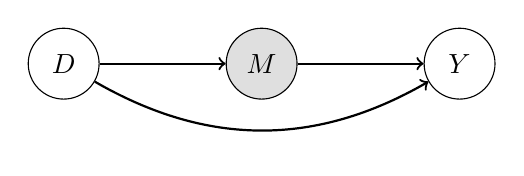
\begin{tikzpicture}[node distance=16mm]
	\node[dag] (D) {$D$};
	\node[dag, right=of D, fill=gray!25] (M) {$M$};
	\node[dag, right=of M] (Y) {$Y$};
	\draw[->, thick] (D) -- (M);
	\draw[->, thick] (M) -- (Y);
	\draw[->, thick] (D) to[bend right=30] (Y);
\end{tikzpicture}
\end{center}
\smallskip
{\small $D$ = thesis, $M$ = first job, $Y$ = earnings}
\end{column}
\begin{column}{0.56\textwidth}
\begin{itemize}
	\item Maybe the thesis raises earnings partly by helping you land a research or consulting job.
	\item ``Controlling for first job'' then \alert{removes part of the effect} you are trying to measure.
	\item Rule: \alert{don't control for outcomes of the treatment}.
	\item Ask of every control: was it determined \alert{before} or \alert{after} the treatment?
\end{itemize}
\end{column}
\end{columns}
\end{frame}


\begin{frame}{Bad control \#2: who ends up in your sample}
\begin{columns}
\begin{column}{0.42\textwidth}
\begin{center}
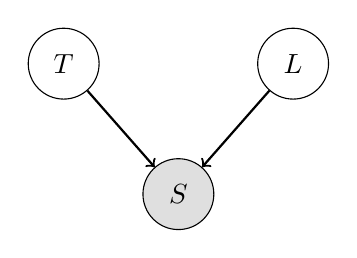
\begin{tikzpicture}[node distance=20mm]
	\node[dag] (T) {$T$};
	\node[dag, right=of T] (L) {$L$};
	\node[dag, below=12mm of $(T)!0.5!(L)$, fill=gray!25] (S) {$S$};
	\draw[->, thick] (T) -- (S);
	\draw[->, thick] (L) -- (S);
\end{tikzpicture}
\end{center}
\smallskip
{\small $T$ = talent, $L$ = luck, $S$ = startup gets funded}
\end{column}
\begin{column}{0.56\textwidth}
\begin{itemize}
	\item Talent and luck are unrelated in the population.
	\item Among \alert{funded startups} they are negatively related: a funded founder who isn't talented must have been lucky.
	\item Restricting your sample to $S$ \alert{creates} a correlation that isn't there. $S$ is called a \alert{collider}.
	\item Thesis version: studying only students who got Wall Street offers. Both the thesis and unobserved talent helped get them there.
\end{itemize}
\end{column}
\end{columns}
\end{frame}


\begin{frame}{A field guide to controls}
\begin{center}
\small
\begin{tabular}{lll}
\toprule
The variable is\ldots & Control for it? & Why \\
\midrule
A common cause of $D$ and $Y$ & \alert{Yes} & blocks a backdoor \\
A rough proxy for one & Usually & blocks it partially \\
A predictor of $Y$ only (pre-treatment) & Yes & smaller standard errors \\
Caused by the treatment & \alert{No} & removes part of the effect \\
Caused by both $D$ and $Y$ (or defines your sample) & \alert{No} & creates bias \\
\bottomrule
\end{tabular}
\end{center}
\bigskip
\begin{itemize}
	\item ``Add every control you have'' is \alert{not} a safe default.
	\item Further reading: Cinelli, Forney \& Pearl (2022), ``A Crash Course in Good and Bad Controls.''
\end{itemize}
\end{frame}


% =====================================================================
\section{Selection on Observables}
% =====================================================================

\begin{frame}{Matching: compare like with like}
Thesis writers have better grades, take harder classes, have better recommendations\ldots
\begin{itemize}
	\item \alert{Matching}: for each thesis writer, find a non-writer with the same GPA, major, test scores, etc. Use them as the counterfactual.
	\item Easy with a few variables. With many, you need to decide what ``close'' means (nearest neighbors, propensity scores, weighting).
	\item Always show a \alert{balance table}: after matching, do the two groups look alike on what you observe?
\end{itemize}
\medskip
Tools: \texttt{MatchIt} and \texttt{cobalt} in R; \texttt{teffects} in Stata.
\end{frame}


\begin{frame}{The limits of matching}
Matching assumes \alert{all} differences between writers and non-writers are captured by what you observe.
\begin{itemize}
	\item No \alert{selection on unobservables}: ambition, curiosity, who your advisor knows\ldots
	\item ``Counterfactual you'' = someone with your grades and test scores who chose not to write a thesis. Why did they choose that?
\end{itemize}
\medskip
What helps:
\begin{itemize}
	\item Use what you know about \alert{how treatment was assigned}. Suppose only students \emph{invited} to write a thesis can. Now compare invited students who wrote to invited students who didn't.
	\item \alert{Sensitivity analysis}: how strong would an unobserved confounder have to be to explain away your result? (Oster 2019; Cinelli \& Hazlett 2020, \texttt{sensemakr}.)
\end{itemize}
\medskip
Usually the better answer is a \alert{research design} that doesn't rely on having measured everything.
\end{frame}


\begin{frame}{Where do counterfactuals come from?}
\small
\begin{tabularx}{\textwidth}{>{\raggedright}p{2.6cm}>{\raggedright}X>{\raggedright\arraybackslash}X}
\toprule
Design & Counterfactual is\ldots & You must believe\ldots \\
\midrule
Experiment / lottery & people who lost the coin flip & assignment really was random \\
Instrumental variables & people pushed away from treatment by something unrelated to $Y$ & the push affects $Y$ only through $D$ \\
Event study & the same unit before the event & nothing else changed at that moment \\
Difference-in-differences & the change in an untreated group & trends would have been parallel \\
Synthetic control & a weighted mix of untreated units & the mix tracks the treated unit \\
Regression discontinuity & units just on the other side of a cutoff & nothing else jumps at the cutoff \\
\bottomrule
\end{tabularx}
\end{frame}


% =====================================================================
\section{Lotteries and Natural Experiments}
% =====================================================================

\begin{frame}{Experiments someone else ran}
\begin{itemize}
	\item What about an \alert{actual experiment} that someone else ran for other reasons?
	\item Or something that isn't an experiment but \alert{looks like one}?
	\item We want variation in treatment that is \alert{as good as random}.
\end{itemize}
\end{frame}


\begin{frame}{Angrist, Pathak \& Walters (2013): charter schools}
Do charter schools improve test scores?
\begin{itemize}
	\item \alert{Problem}: families who apply to charters may care more about education. Comparing charter to public school students mixes the school effect with family effort.
	\item \alert{Solution}: popular charters are over-subscribed and admit students by \alert{lottery}.
	\item Compare lottery \alert{winners} to \alert{losers}. Both groups applied, so both care about education. Only luck differs.
\end{itemize}
\end{frame}


\begin{frame}{Angrist, Pathak \& Walters (2013)}
\centering
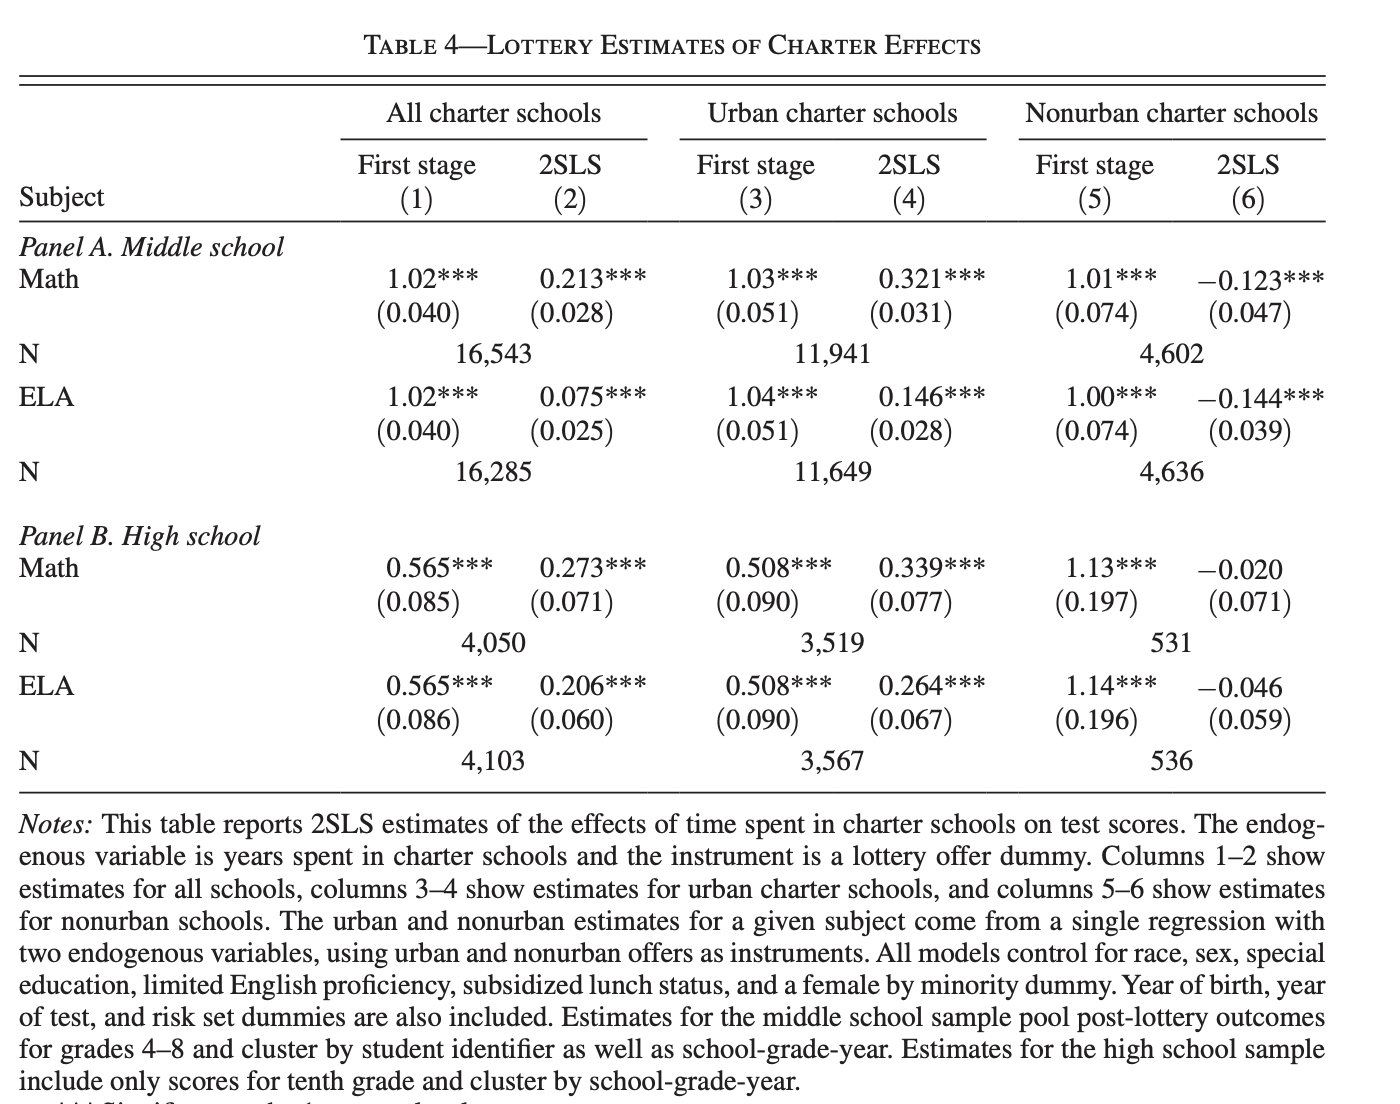
\includegraphics[height=0.85\textheight]{apw_3.png}
\end{frame}


\begin{frame}{How does it work?}
Not every winner attends, and some losers get in later. So scale the effect of \emph{winning}:
\begin{align*}
\text{effect of attending} \;=\;
\frac{\text{score gap between winners and losers}}{\text{attendance gap between winners and losers}}
\end{align*}
\begin{itemize}
	\item If winning raises scores by 0.1 SD and raises attendance by 50 percentage points, then attending raises scores by $0.1/0.5 = 0.2$ SD.
	\item This is \alert{instrumental variables (IV)}. The lottery is the \alert{instrument}.
	\item Two things must hold:
	\begin{enumerate}
		\item The lottery actually changes who attends (\alert{relevance}, which you can check).
		\item The lottery affects scores \alert{only} through attendance (\alert{exclusion}, which you must argue).
	\end{enumerate}
\end{itemize}
\end{frame}


\begin{frame}{Whose effect does IV measure?}
Think about four kinds of applicants:
\begin{center}
\begin{tabular}{lll}
\toprule
Type & If they win & If they lose \\
\midrule
\alert{Always-takers} & attend & attend anyway (sibling, waitlist) \\
\alert{Never-takers} & don't attend & don't attend \\
\alert{Compliers} & attend & don't attend \\
Defiers (assume none) & don't attend & attend \\
\bottomrule
\end{tabular}
\end{center}
\begin{itemize}
	\item The lottery only changes behavior for \alert{compliers}, so IV estimates the effect \alert{for compliers} (a ``local'' average effect, LATE).
	\item A different instrument changes behavior for different people, so it can give a different (equally correct) answer.
\end{itemize}
\end{frame}


\begin{frame}{Other lotteries and near-lotteries}
\begin{itemize}
	\item \alert{Angrist (1990)}: does military service affect later earnings?
	\begin{itemize}
		\item Vietnam draft lottery numbers were random. White veterans earned roughly 15\% less a decade later.
		\item Exclusion worry: did low numbers also push men to stay in school to avoid the draft?
	\end{itemize}
	\item \alert{Judge designs}: cases are randomly assigned to judges, and some judges are harsher than others.
	\begin{itemize}
		\item Dobbie, Goldin \& Yang (2018): pretrial detention raises conviction rates and lowers later employment.
		\item The same idea works for patent examiners, caseworkers, loan officers, and \ldots\ thesis advisors.
	\end{itemize}
	\item \alert{Weather}: storms at sea cut the supply of fish at the Fulton Fish Market, which traces out demand (Graddy 2006).
\end{itemize}
\medskip
In every case, ask: \alert{could the instrument affect the outcome some other way?}
\end{frame}


\begin{frame}{Sinkinson \& Starc (2019): do drug ads work?}
\begin{itemize}
	\item \alert{Problem}: firms set ad budgets as a share of revenue, and advertise where they expect ads to work. Ads and sales move together for reasons other than ads causing sales.
	\item \alert{Idea}: during election season, political ads crowd out TV ad slots, so cholesterol-drug ads get displaced.
	\item Crowding out is worse in \alert{swing states} and around \alert{primaries}, and has nothing to do with how well drug ads work.
	\item That moves drug ads around for reasons \alert{unrelated to drug demand}: an instrument.
\end{itemize}
\end{frame}


\begin{frame}{Sinkinson \& Starc (2019): political ads crowd out drug ads}
\begin{columns}
\begin{column}{0.5\textwidth}
\centering
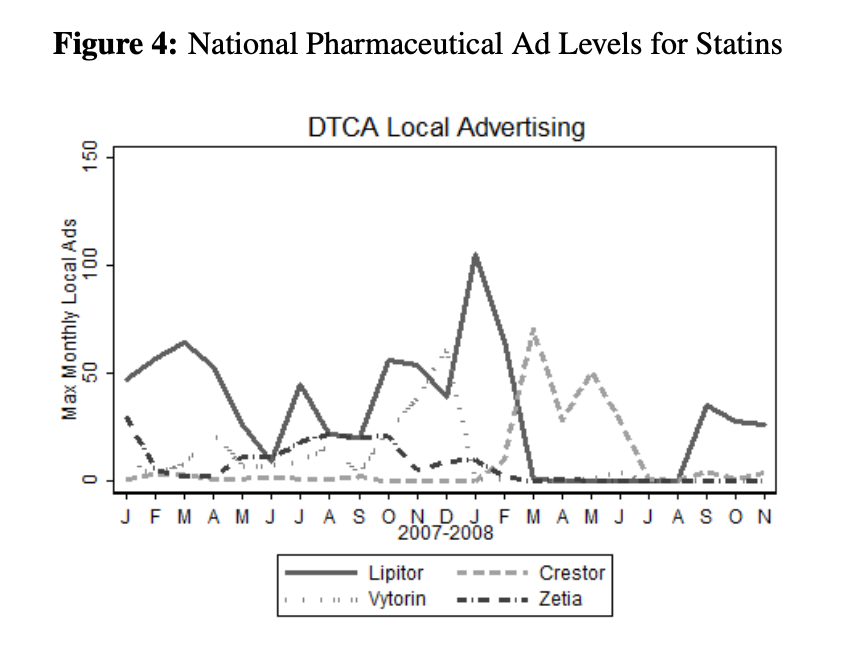
\includegraphics[width=\textwidth]{ss_3.png}
\end{column}
\begin{column}{0.5\textwidth}
\centering
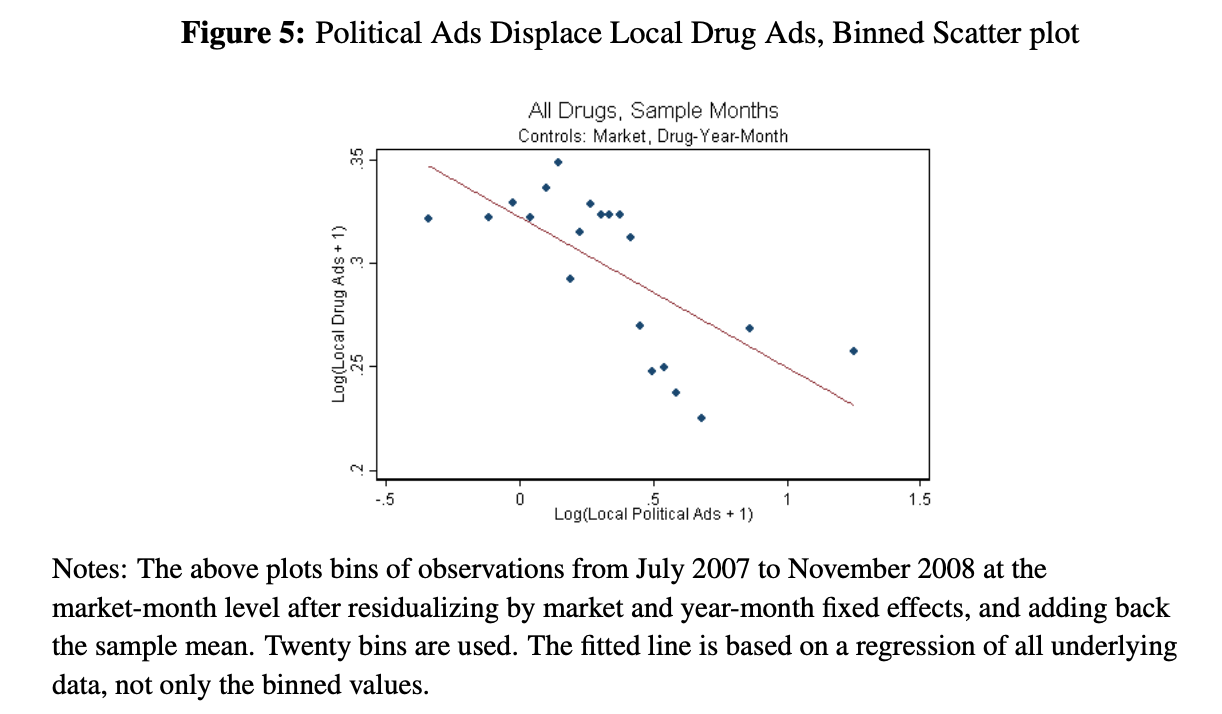
\includegraphics[width=\textwidth]{ss_4.png}
\end{column}
\end{columns}
\end{frame}


\begin{frame}{Sinkinson \& Starc (2019): OLS vs.\ IV}
\begin{columns}[t]
\begin{column}{0.5\textwidth}
\centering
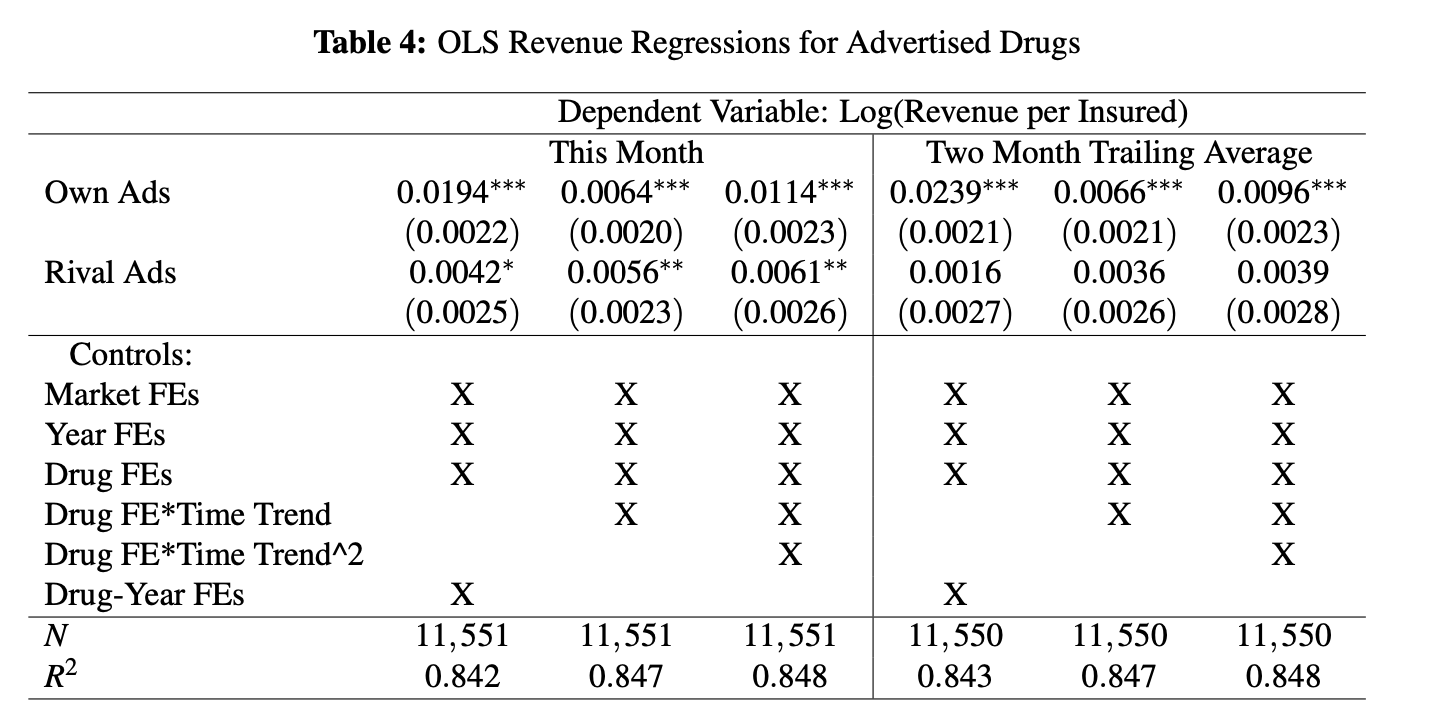
\includegraphics[width=\textwidth]{ss_7.png}
\end{column}
\begin{column}{0.5\textwidth}
\centering
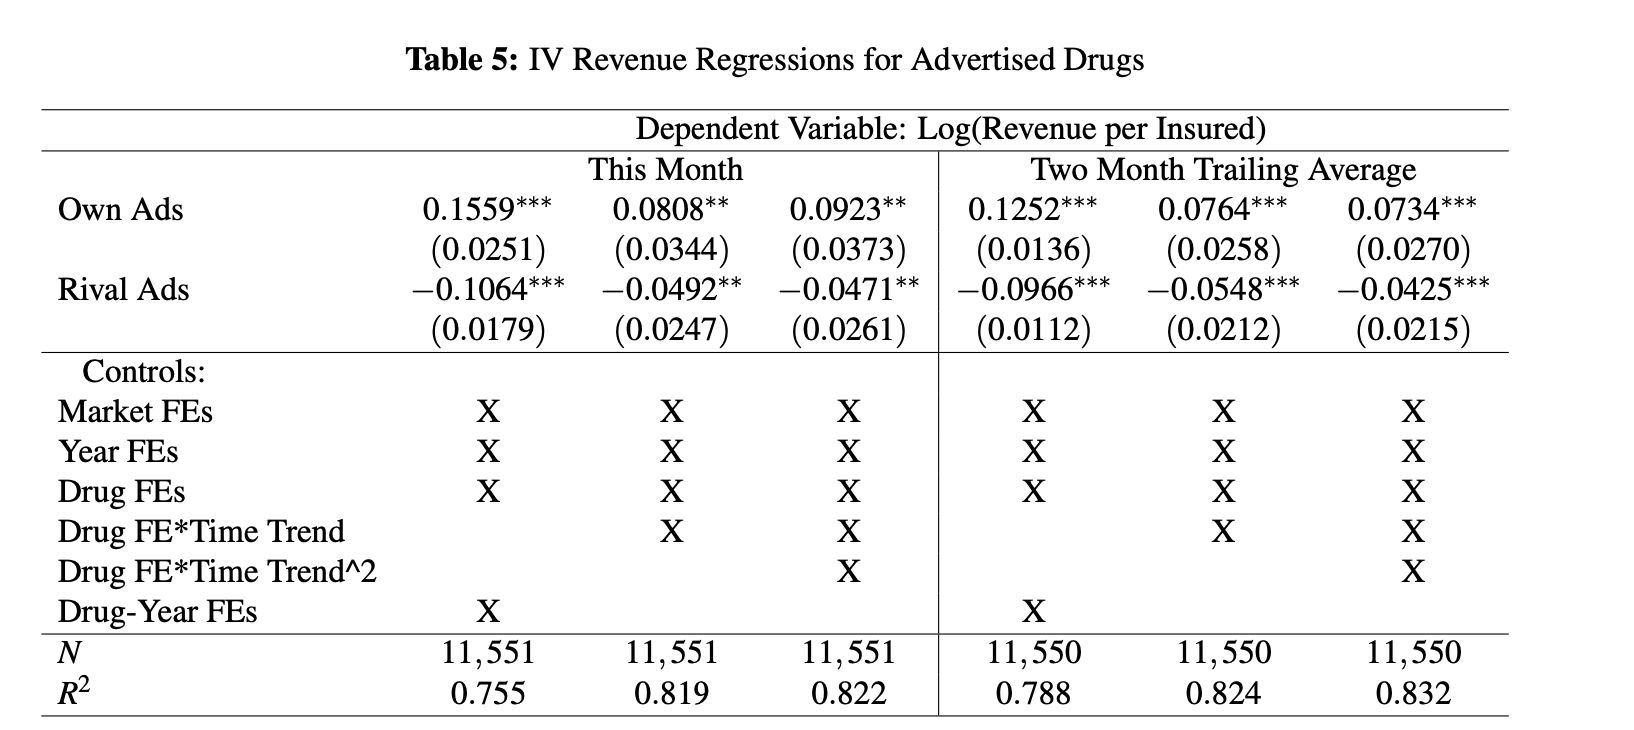
\includegraphics[width=\textwidth]{ss_6.png}
\end{column}
\end{columns}
\medskip
\begin{itemize}
	\item OLS (left): own ads barely matter. IV (right): own ads raise revenue several times more.
	\item With IV, \alert{rival} ads turn negative: one drug's ads steal customers from the others.
	\item OLS was biased toward zero, so the naive comparison \alert{understated} what ads do.
\end{itemize}
\end{frame}


% =====================================================================
\section{Before and After: Event Studies and Difference-in-Differences}
% =====================================================================

\begin{frame}{Using the same unit before and after}
On August 28, 2024, NVIDIA released one of the most anticipated earnings reports ever. What did it do to the stock price?
\begin{itemize}
	\item Counterfactual: the stock's path \alert{just before} the announcement, adjusted for what the overall market did that day.
	\item This is an \alert{event study}. It works when the event is sharp, the window is short, and nothing else happens at the same time.
\end{itemize}
\medskip
For most thesis questions (a policy, a merger, a new law) the window is months or years:
\begin{itemize}
	\item Other things change too: the economy, other policies, trends already under way.
	\item We need someone who \alert{didn't} get treated to tell us what ``other things'' did.
\end{itemize}
\end{frame}


\begin{frame}{Difference-in-differences}
Combine the two counterfactuals: \alert{before vs.\ after} and \alert{treated vs.\ untreated}.
\begin{center}
\begin{tabular}{lccc}
\toprule
 & Before & After & Change \\
\midrule
Treated & $A$ & $B$ & $B - A$ \\
Control & $C$ & $D$ & $D - C$ \\
\midrule
 & & & \alert{$(B-A) - (D-C)$} \\
\bottomrule
\end{tabular}
\end{center}
\begin{itemize}
	\item The control group's change tells us what \alert{would have happened} to the treated group without treatment.
	\item The groups can start at different \alert{levels}. They only need to be on the same \alert{trend}.
\end{itemize}
\end{frame}


\begin{frame}{The classic example: Card \& Krueger (1994)}
\begin{columns}
\begin{column}{0.45\textwidth}
\begin{itemize}
	\item April 1992: New Jersey raises its minimum wage from \$4.25 to \$5.05. Eastern Pennsylvania doesn't.
	\item Survey fast-food restaurants on both sides of the border before and after.
	\item Econ 101 predicts NJ employment falls relative to PA. It didn't.
	\item Decades of debate followed, about data, samples, and whether PA is the right control.
\end{itemize}
\end{column}
\begin{column}{0.55\textwidth}
\centering
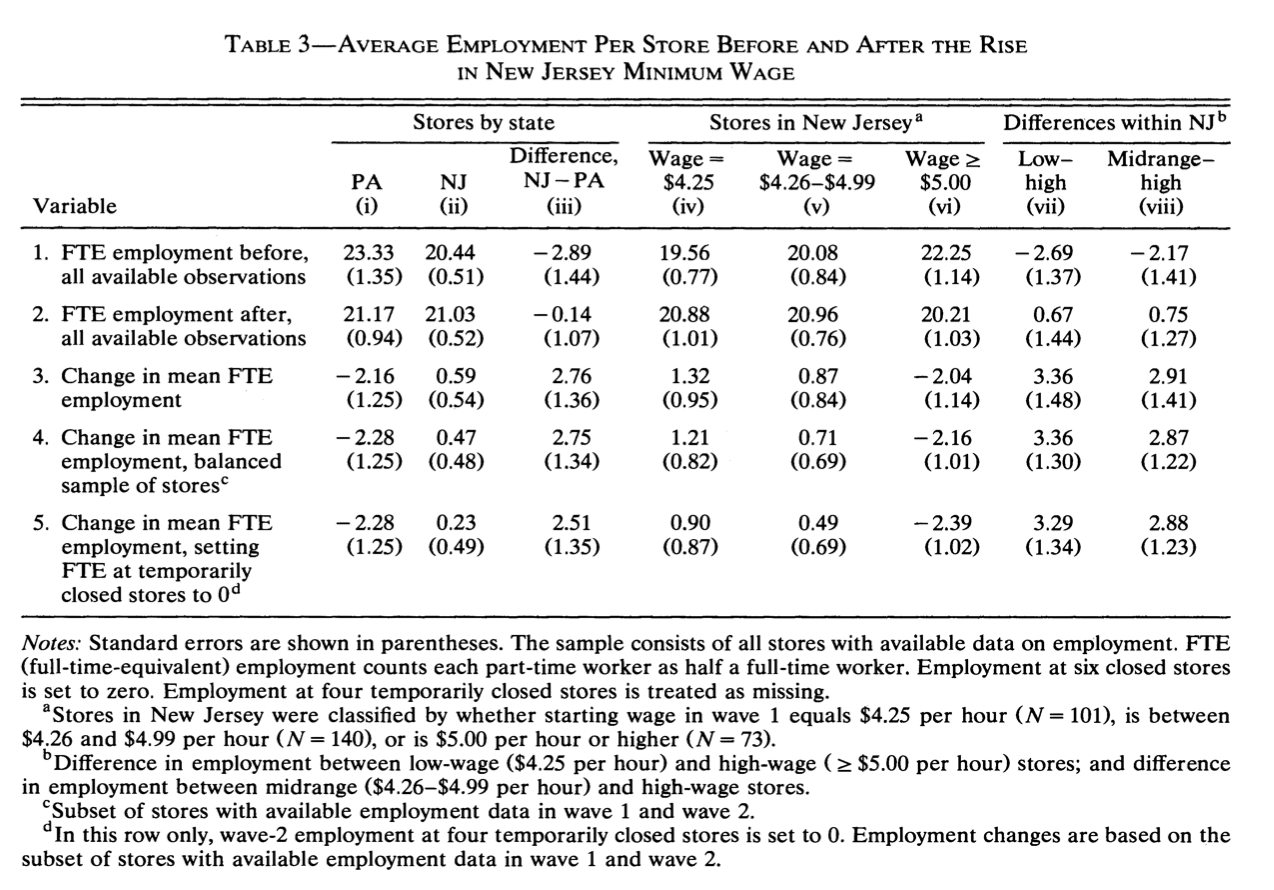
\includegraphics[width=\textwidth]{ck_tab3.png}
\end{column}
\end{columns}
\end{frame}


\begin{frame}{The key assumption: parallel trends}
\begin{columns}
\begin{column}{0.55\textwidth}
\centering
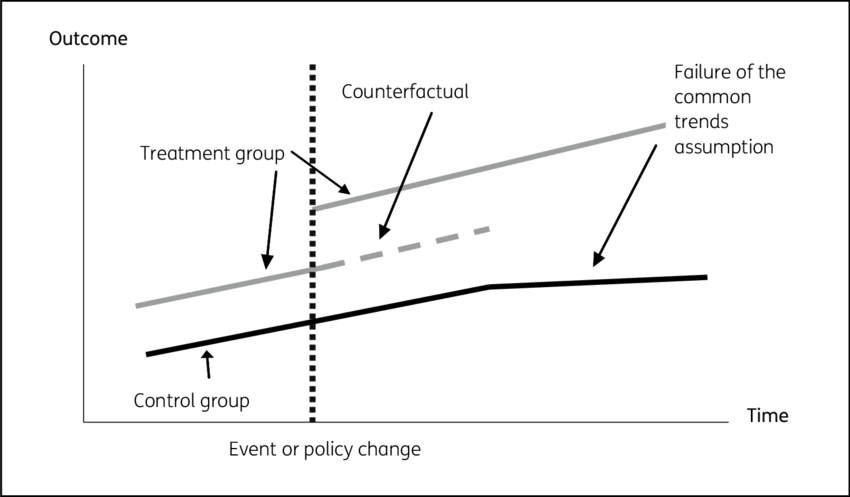
\includegraphics[width=\textwidth]{common_trend.png}
\end{column}
\begin{column}{0.43\textwidth}
\begin{itemize}
	\item Without treatment, the treated group would have followed the \alert{same trend} as the control group.
	\item It is about the post-period \alert{counterfactual}, which we never see. You \alert{cannot test it}, only make it plausible.
	\item Choose controls that face the \alert{same shocks}: neighboring states, similar firms, the same market.
\end{itemize}
\end{column}
\end{columns}
\end{frame}


\begin{frame}{The modern way to show a DiD: the event-study plot}
\begin{columns}
\begin{column}{0.55\textwidth}
\centering
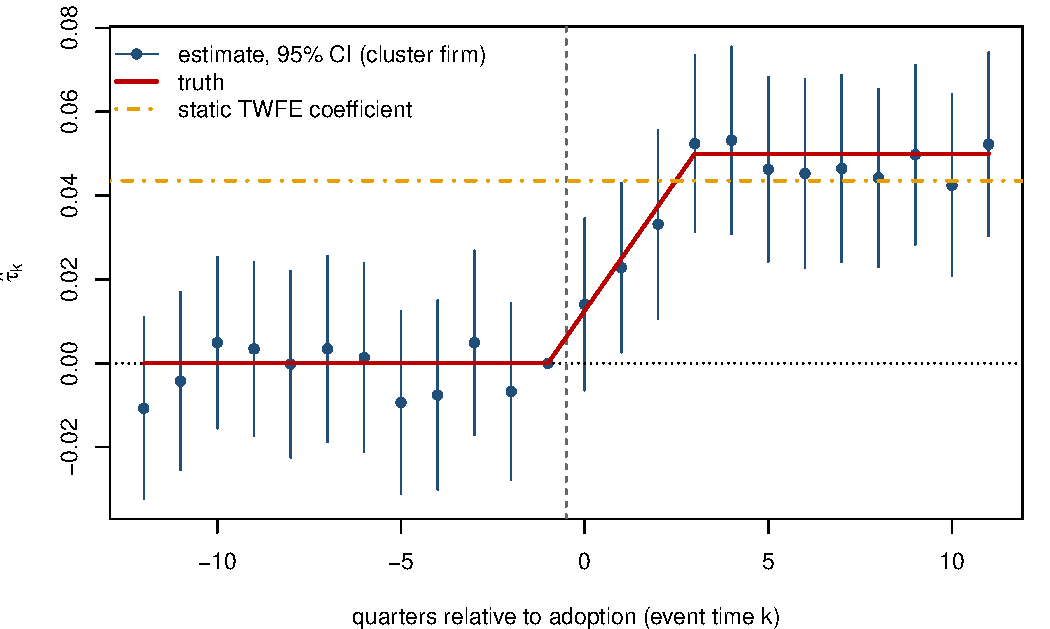
\includegraphics[width=\textwidth]{fig_es_single.pdf}
\end{column}
\begin{column}{0.43\textwidth}
\small
\begin{itemize}
	\item One DiD estimate per period, relative to the period just before treatment ($k=-1$, zero by construction).
	\item \alert{Left of the line}: were treated units already diverging? Should be flat.
	\item \alert{Right of the line}: how the effect evolves. Does it ramp up? Fade out?
	\item A single DiD number averages over this path. Show the path.
\end{itemize}
\end{column}
\end{columns}
{\footnotesize Simulated data: 400 firms adopt a pricing tool in quarter 13; true effect in red.}
\end{frame}


\begin{frame}{Flat pre-trends do not prove parallel trends}
\begin{columns}
\begin{column}{0.55\textwidth}
\centering
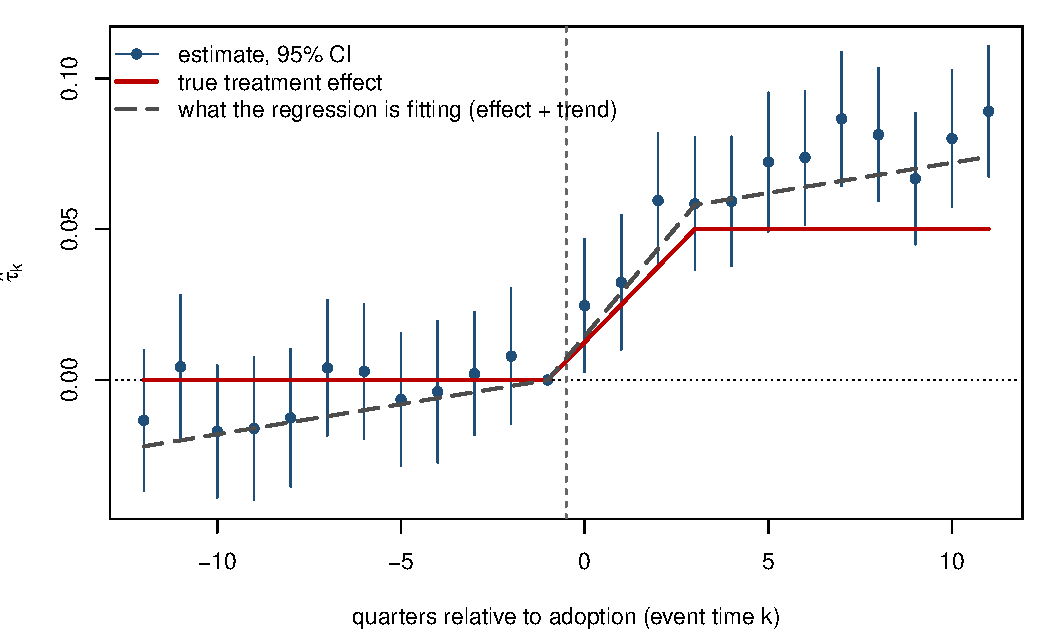
\includegraphics[width=\textwidth]{fig_es_pretrend.pdf}
\end{column}
\begin{column}{0.43\textwidth}
\small
\begin{itemize}
	\item Same data plus a small extra trend for treated firms. No pre-period estimate is significant, but every post-period estimate is \alert{too big}.
	\item ``The pre-trends are insignificant'' is weak evidence. A noisy test passes easily (Roth 2022).
	\item Better: say how big a trend your data can rule out, and how much it could move your answer (Rambachan \& Roth 2023, \texttt{HonestDiD}).
\end{itemize}
\end{column}
\end{columns}
\end{frame}


\begin{frame}{What breaks parallel trends?}
\begin{enumerate}
	\item \alert{Something else changed at the same time.} If NJ raised the minimum wage because a new governor arrived with a whole package of policies, NJ and PA diverge for other reasons too, even if they tracked each other before.
	\item \alert{Selection on a temporary dip.} People join job training after a bad year. Their earnings would have bounced back anyway (next slide).
	\item \alert{Anticipation.} Firms react to a law when it is announced, not when it takes effect.
	\item \alert{Composition.} Treatment changes who is in the sample: restaurants close in NJ and reopen in PA, or workers move.
\end{enumerate}
\medskip
For each, ask: \alert{why did this unit get treated at this time?}
\end{frame}


\begin{frame}{The ``Ashenfelter dip'' (Heckman \& Smith 1999)}
\begin{columns}
\begin{column}{0.55\textwidth}
\centering
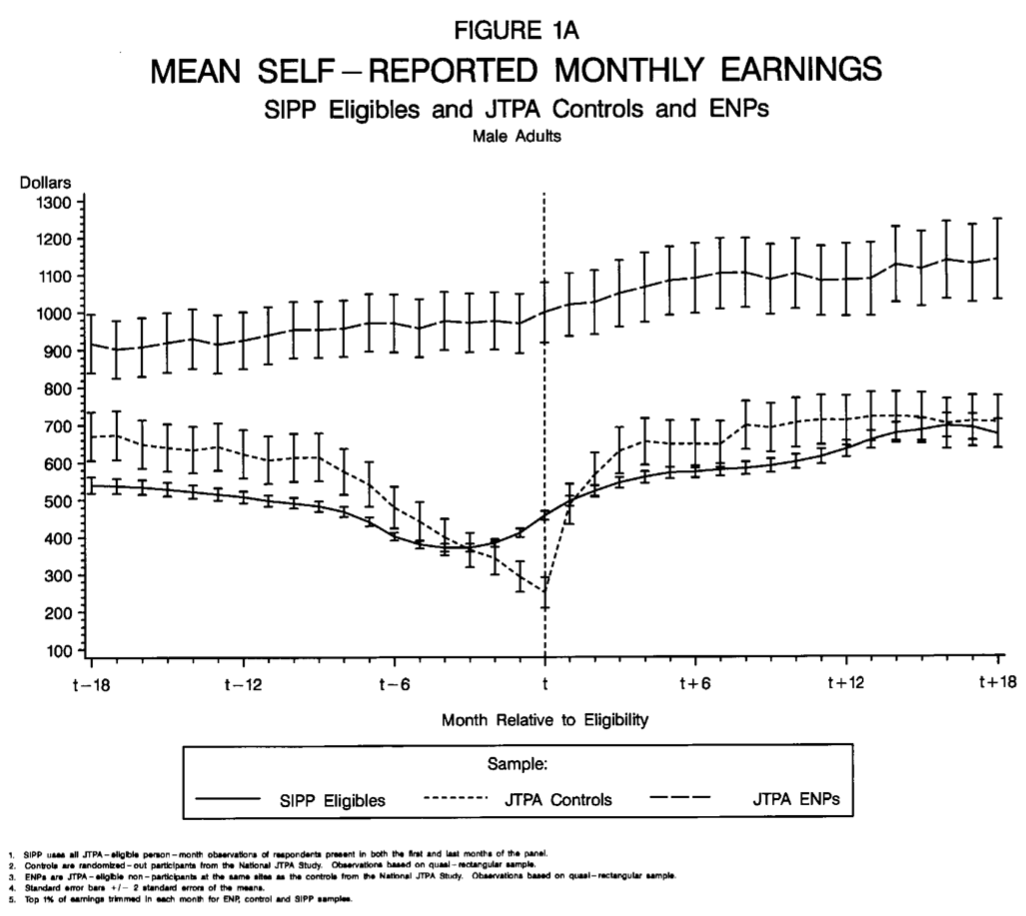
\includegraphics[width=\textwidth]{ashenfelter_dip.png}
\end{column}
\begin{column}{0.43\textwidth}
\begin{itemize}
	\item Earnings of job-training participants \alert{drop} just before they enroll.
	\item Some of the rebound afterwards would have happened anyway (\alert{regression to the mean}).
	\item DiD starting from the dip overstates the program's effect.
\end{itemize}
\end{column}
\end{columns}
\end{frame}


\begin{frame}{Staggered adoption: when treatment arrives at different times}
Most policies roll out \alert{gradually}: states adopt a law in different years, firms adopt a technology one by one.
\begin{itemize}
	\item Example: U.S. states adopted unilateral (no-fault) divorce between 1969 and 1985. Did it change female suicide rates? (Stevenson \& Wolfers 2006)
	\item Standard approach until about 2020: regress the outcome on a treatment dummy with state and year fixed effects (``two-way fixed effects'').
	\item It seems strictly better than one treated state. It isn't automatically.
\end{itemize}
\medskip
Since 2020, a large literature (Goodman-Bacon; Callaway \& Sant'Anna; Sun \& Abraham; de Chaisemartin \& D'Haultf{\oe}uille; Borusyak, Jaravel \& Spiess) shows \alert{what that regression actually compares}.
\end{frame}


\begin{frame}{Three groups: early, late, never treated}
\centering
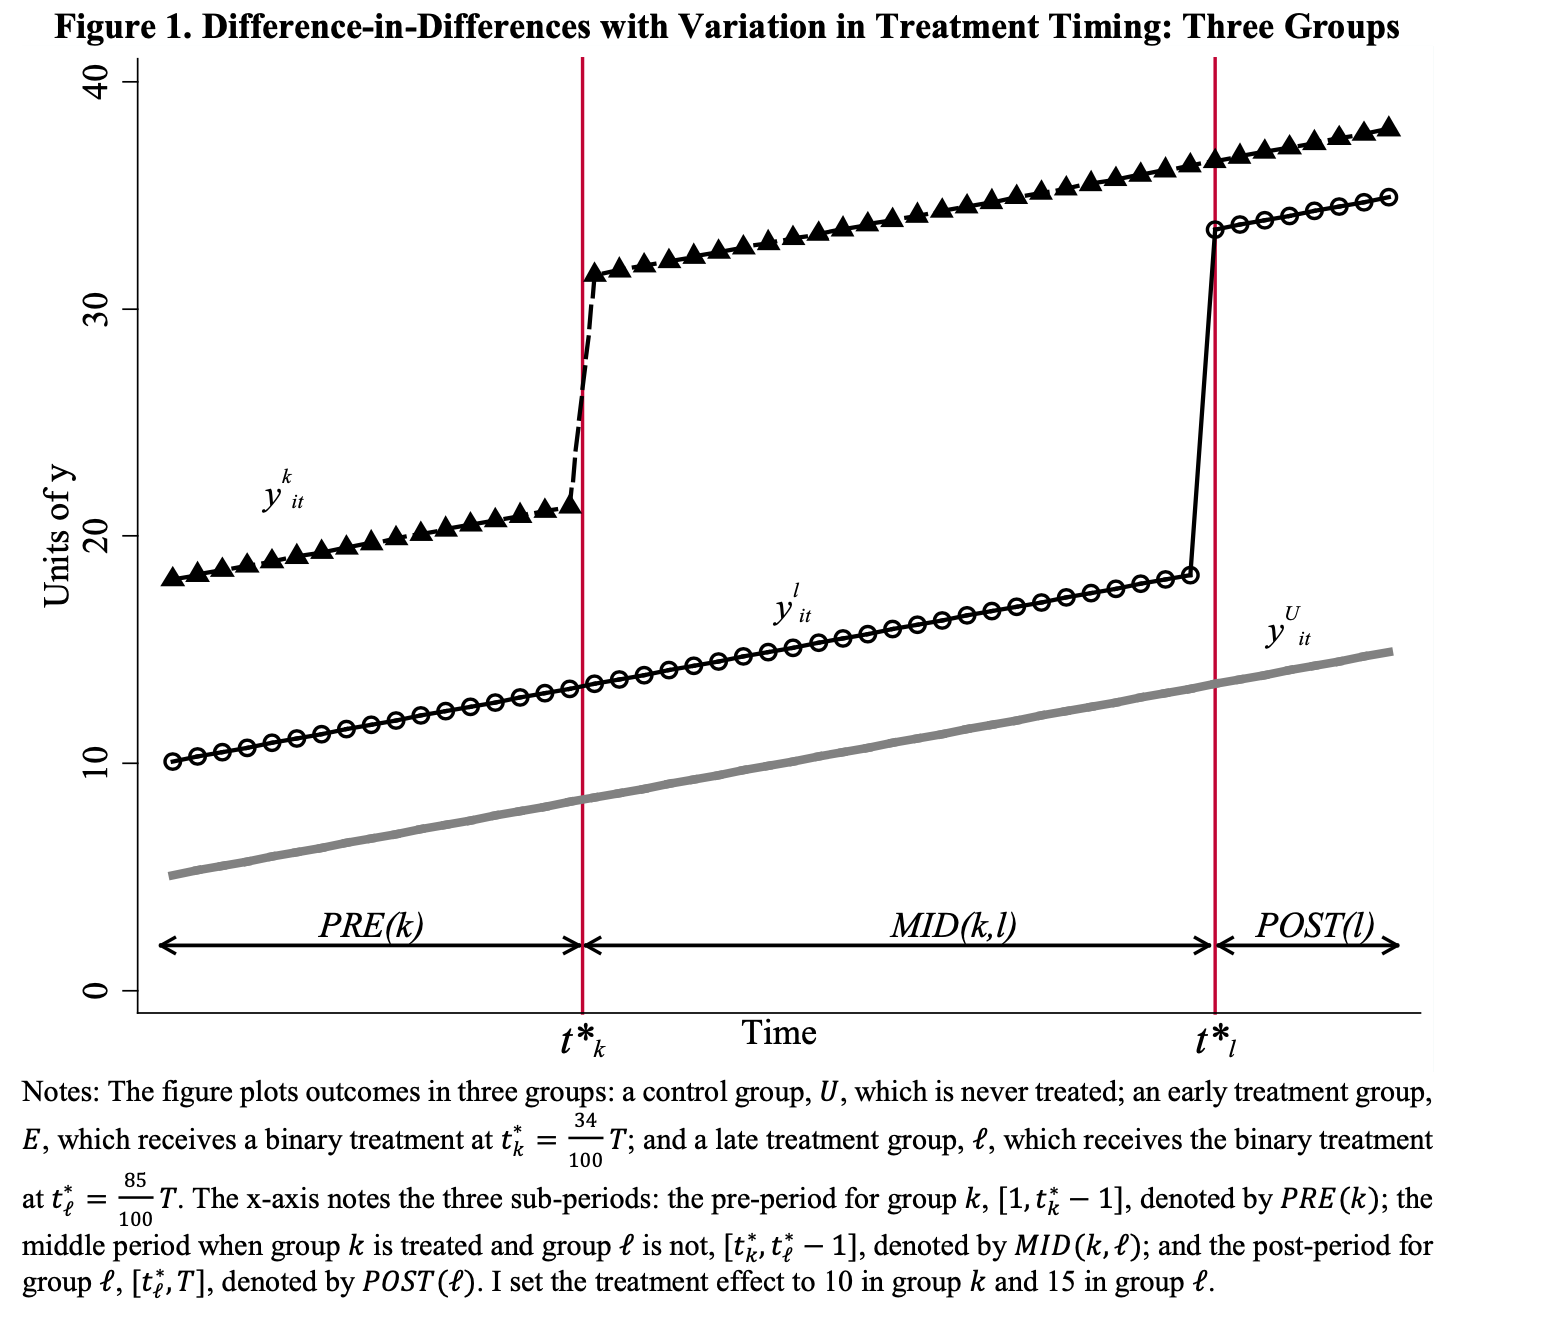
\includegraphics[height=0.85\textheight]{gb_fig1.png}
\end{frame}


\begin{frame}{What the regression secretly compares (Goodman-Bacon 2021)}
\begin{columns}
\begin{column}{0.5\textwidth}
\centering
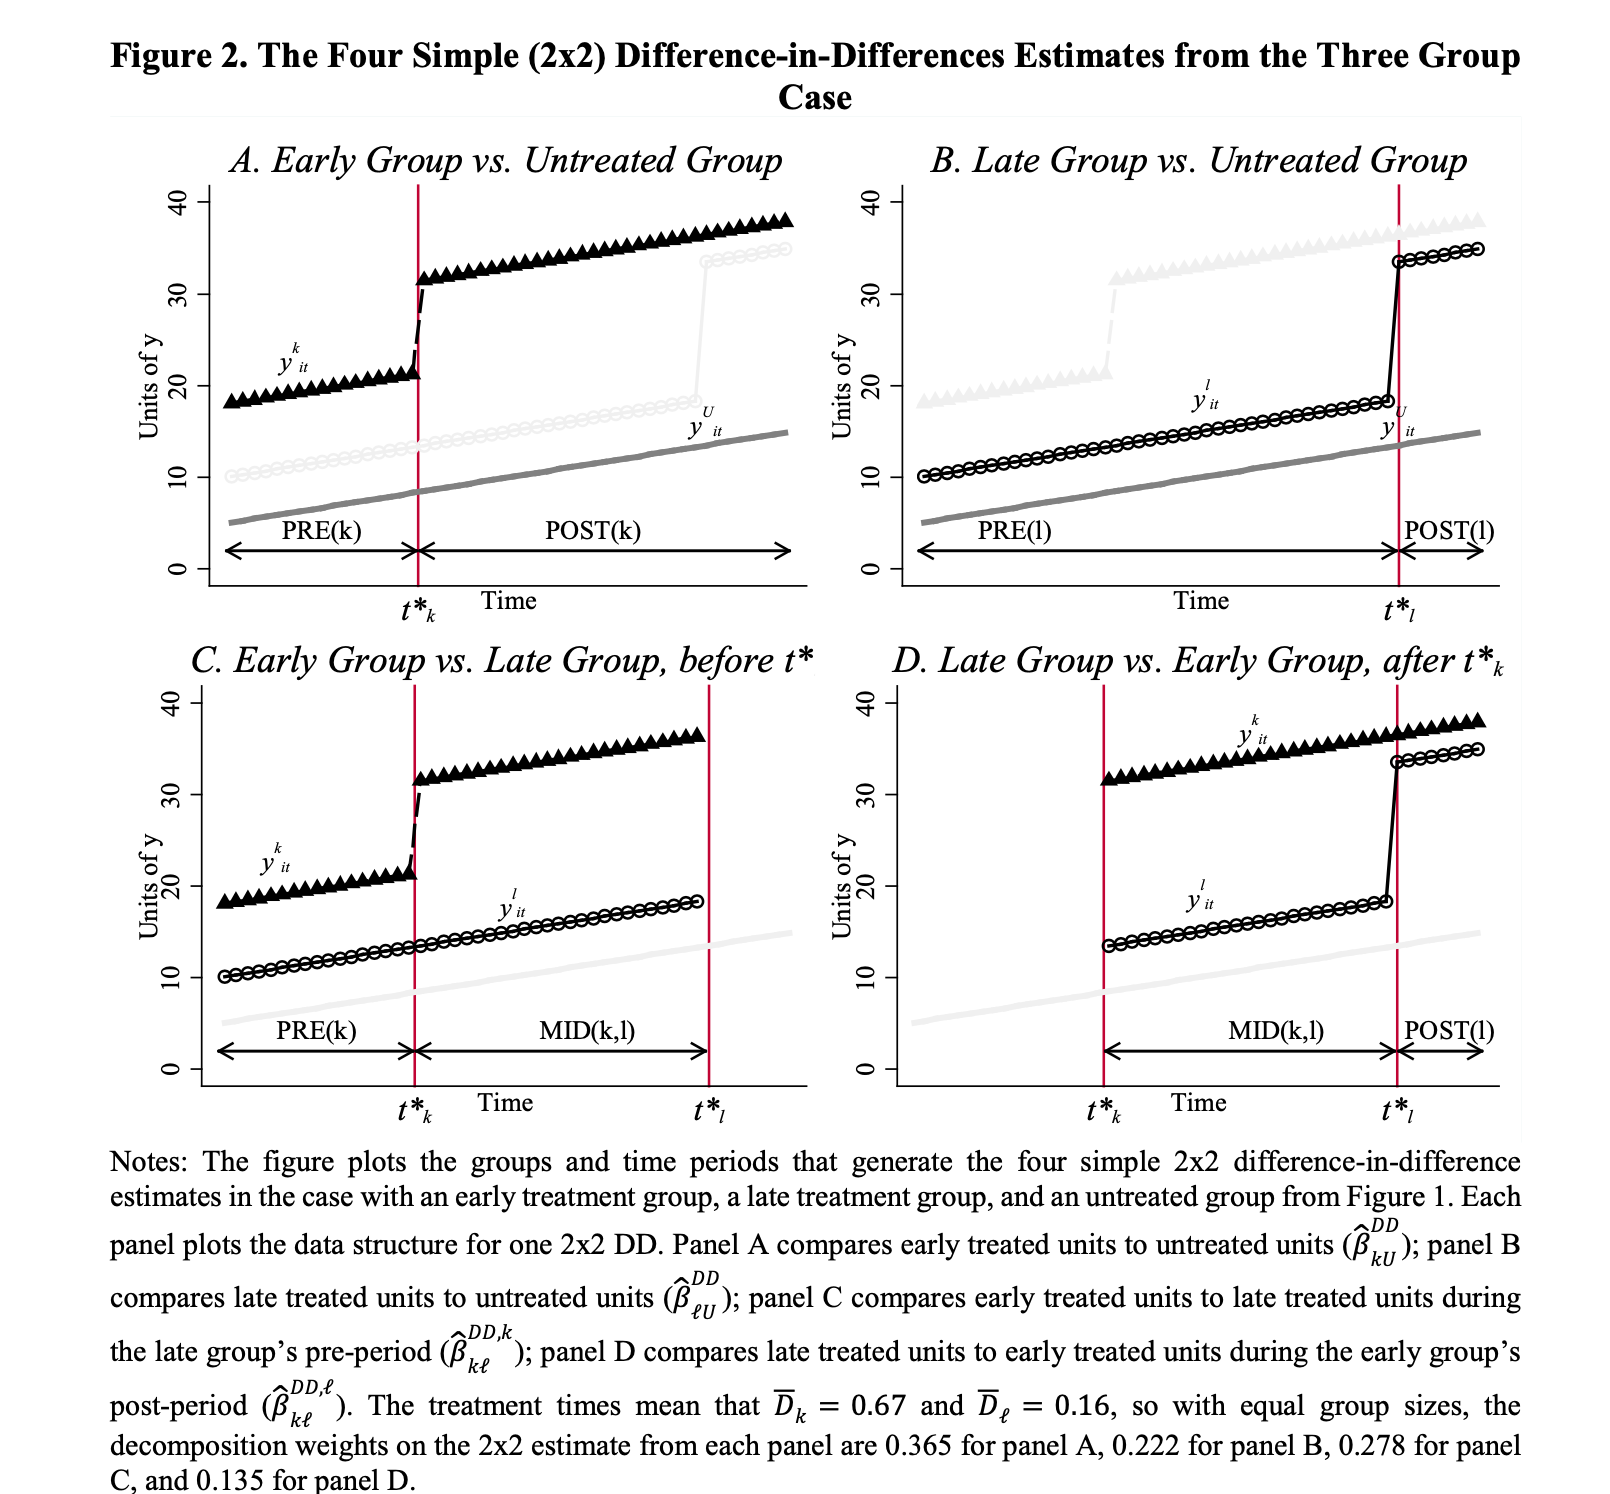
\includegraphics[height=0.78\textheight]{gb_fig2.png}
\end{column}
\begin{column}{0.48\textwidth}
The regression averages every possible $2\times2$ DiD:
\begin{itemize}
	\item[A.] Early vs.\ never treated \hfill \alert{fine}
	\item[B.] Late vs.\ never treated \hfill \alert{fine}
	\item[C.] Early vs.\ late, before the late group is treated \hfill \alert{fine}
	\item[D.] Late vs.\ early, \emph{after} the early group is treated \hfill \alert{problem}
\end{itemize}
\medskip
In D, an \alert{already-treated} group serves as the control.
\end{column}
\end{columns}
\end{frame}


\begin{frame}{Why comparison D is a problem}
\begin{columns}
\begin{column}{0.5\textwidth}
\centering
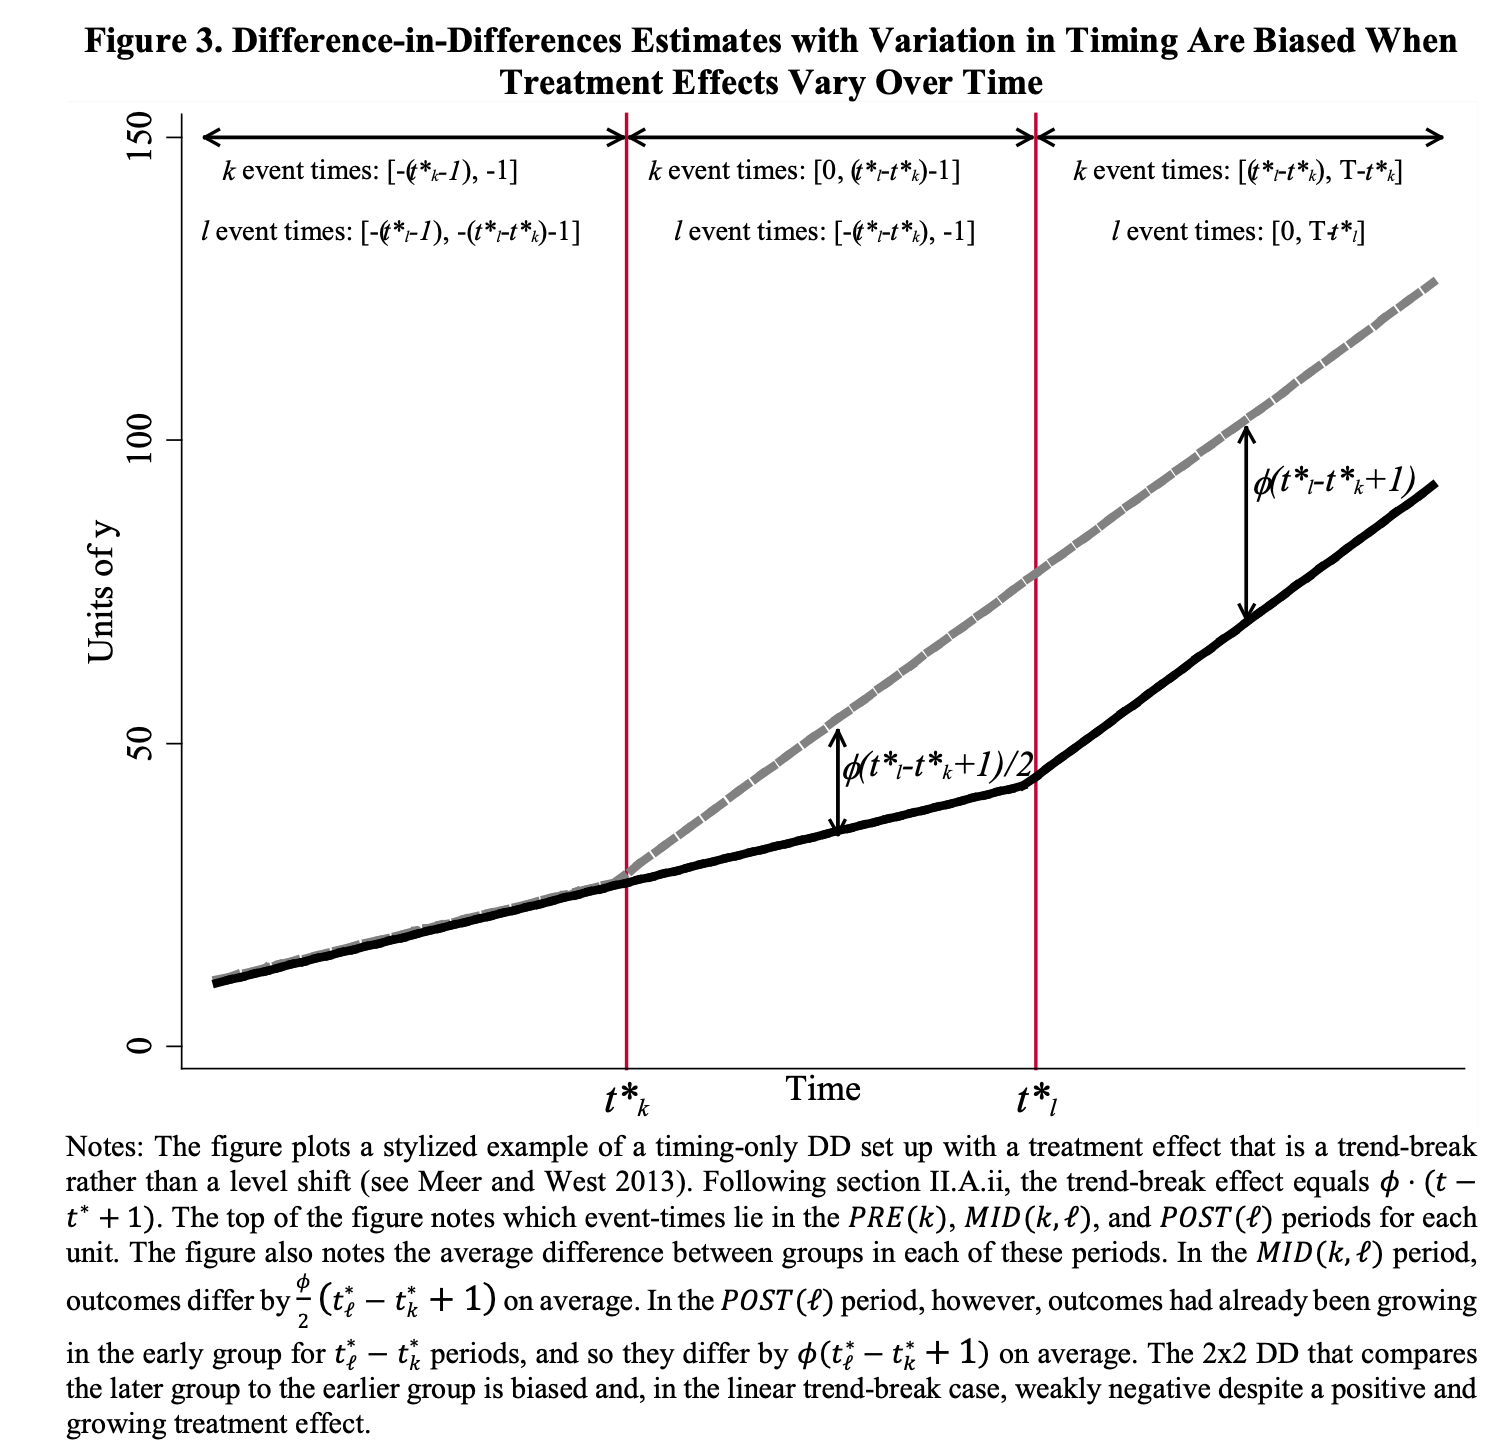
\includegraphics[height=0.78\textheight]{gb_fig3.png}
\end{column}
\begin{column}{0.48\textwidth}
\begin{itemize}
	\item If the effect \alert{grows over time}, the early group is still changing because of \emph{its own} treatment.
	\item Using it as a control subtracts part of the treatment effect.
	\item The overall estimate can be badly biased, and even have the \alert{wrong sign}, though every unit's effect is positive.
\end{itemize}
\end{column}
\end{columns}
\end{frame}


\begin{frame}{The fix: only make clean comparisons}
The idea behind the modern estimators is simple:
\begin{enumerate}
	\item For each \alert{cohort} (units treated in the same year), estimate a separate DiD using only \alert{never-treated} or \alert{not-yet-treated} units as controls.
	\item Then \alert{average} those clean estimates yourself: by cohort, by calendar year, or by time since treatment (an event-study plot).
\end{enumerate}
\medskip
\begin{itemize}
	\item R: \texttt{did} (Callaway \& Sant'Anna), \texttt{fixest::sunab} (Sun \& Abraham), \texttt{didimputation}. Stata: \texttt{csdid}, \texttt{did\_imputation}, \texttt{jwdid}.
	\item If everyone is treated at the same time, the classic regression is fine. If timing varies, \alert{use one of these}.
\end{itemize}
\end{frame}


\begin{frame}{Event study done right: no-fault divorce}
\centering
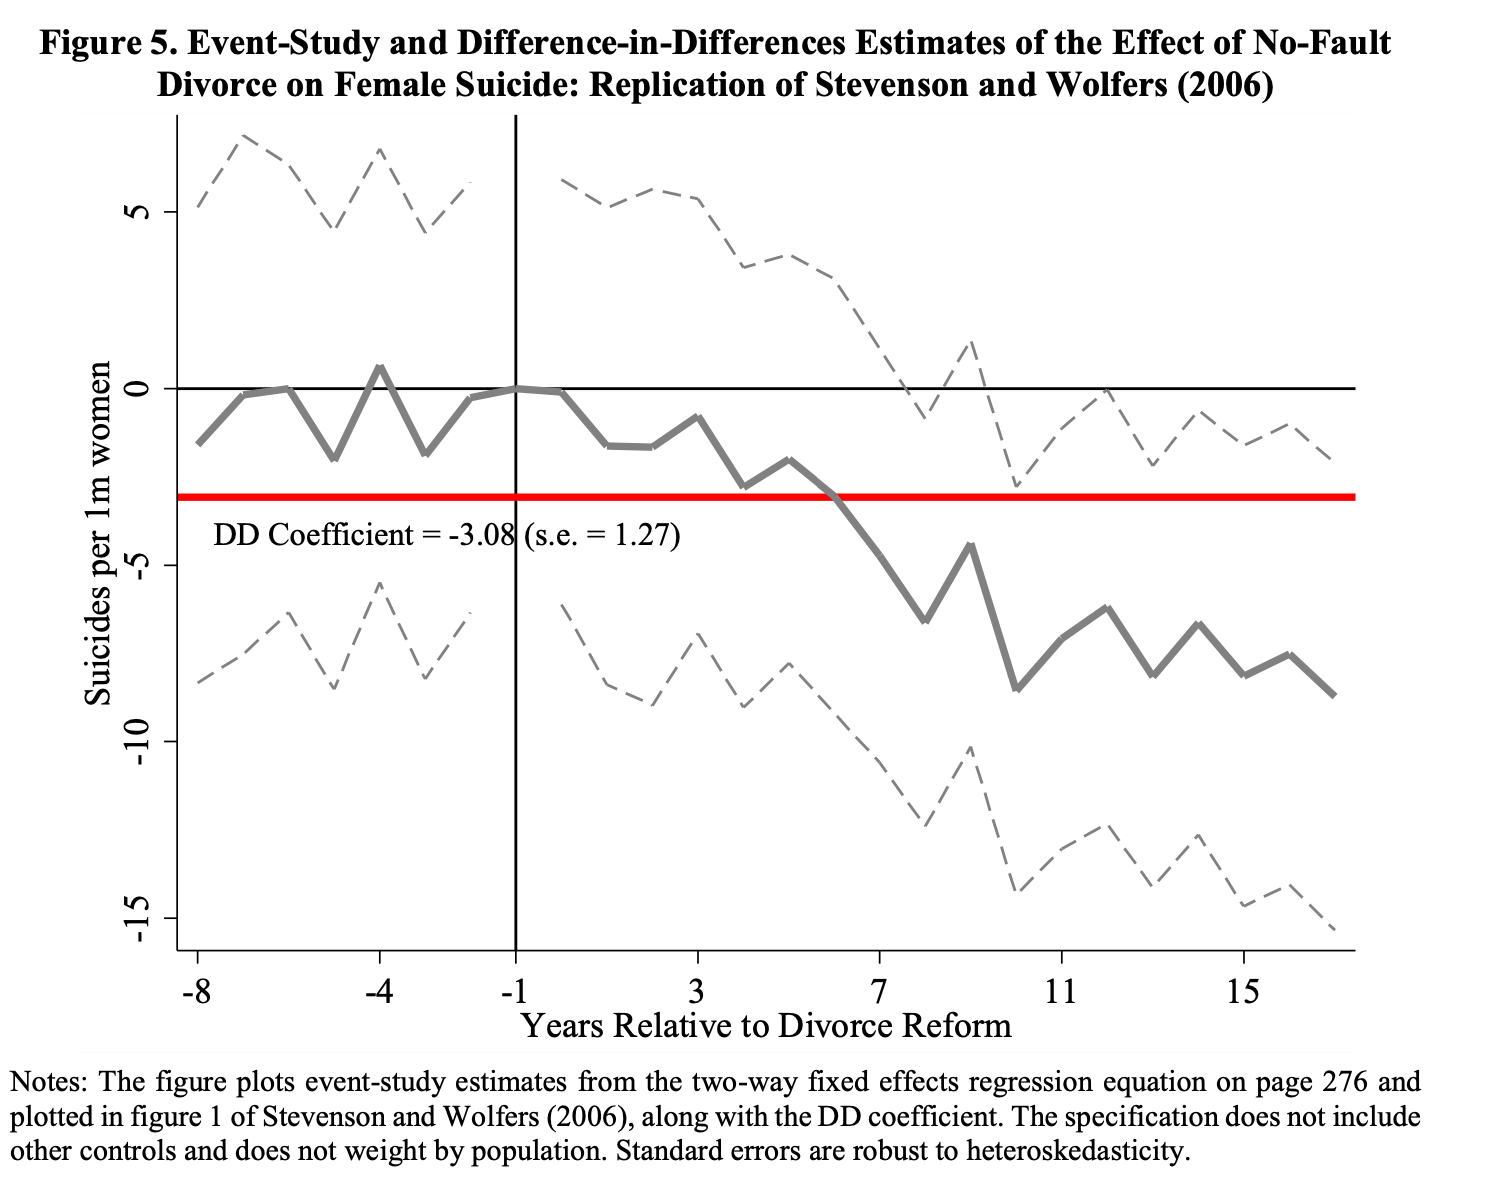
\includegraphics[height=0.85\textheight]{gb_fig5.png}
\end{frame}


\begin{frame}{A DiD checklist for your thesis}
\begin{enumerate}
	\item Who is treated, who is the control, and \alert{when} does treatment start?
	\item \alert{Why} did treated units get treated at that time? Is that reason related to the outcome?
	\item Plot the \alert{raw averages} for each group over time before running any regression.
	\item Show the \alert{event-study plot}. Discuss how big a pre-trend you could have missed.
	\item If timing is \alert{staggered}, use a modern estimator, not plain two-way fixed effects.
	\item Cluster standard errors at the level treatment is assigned (states, not people). With only a few treated states, be humble about precision.
\end{enumerate}
\end{frame}


% =====================================================================
\section{One Treated Unit: Synthetic Control}
% =====================================================================

\begin{frame}{Abadie, Diamond \& Hainmueller (2010): California's Prop 99}
In 1988 California passed Proposition 99:
\begin{itemize}
	\item Raised the cigarette tax by 25 cents per pack
	\item Funded anti-smoking education and ads
	\item Followed by local indoor smoking bans
\end{itemize}
What was the effect on cigarette sales per person?
\begin{itemize}
	\item Only \alert{one} treated state, and sales were already falling everywhere.
	\item Which state is a good control for California? Nevada? Oregon? None of them is very good on its own.
\end{itemize}
\end{frame}


\begin{frame}{The idea: build a ``synthetic California''}
\begin{itemize}
	\item Take a \alert{weighted average of other states} that matches California's cigarette sales \alert{every year before 1988}, and its income, prices, and demographics.
	\item Weights are non-negative and add to one. The data choose them, not you.
	\item After 1988, the gap between real and synthetic California is the estimated effect.
\end{itemize}
\medskip
\begin{itemize}
	\item Like \alert{matching}: build a control that looks like the treated unit.
	\item Like \alert{DiD}: compare paths before and after.
	\item Credibility comes from \alert{how well the pre-period fits}, so show it.
\end{itemize}
\end{frame}


\begin{frame}{Synthetic California}
\begin{columns}
\begin{column}{0.5\textwidth}
\centering
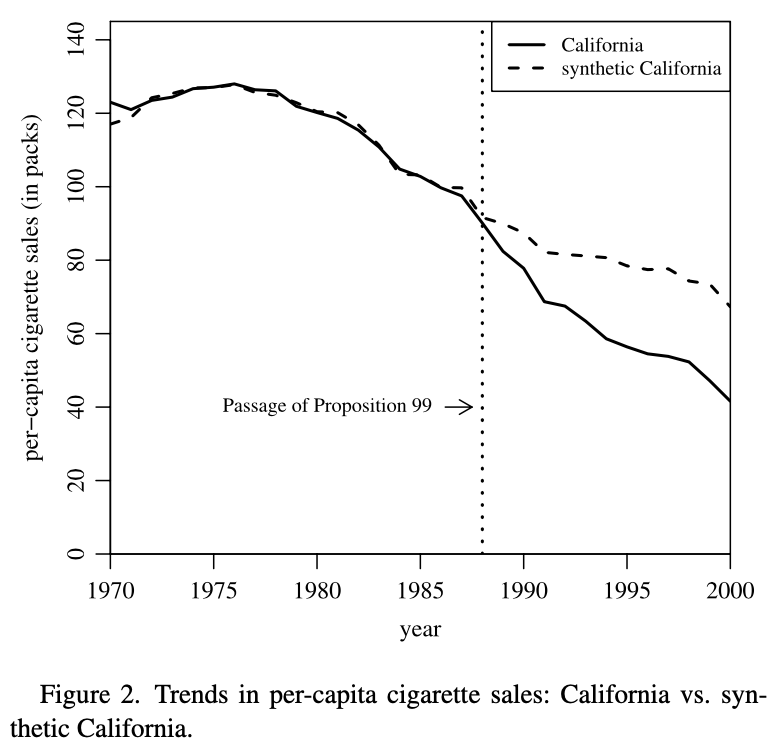
\includegraphics[height=0.66\textheight]{abadie_3.png}
\end{column}
\begin{column}{0.5\textwidth}
\centering
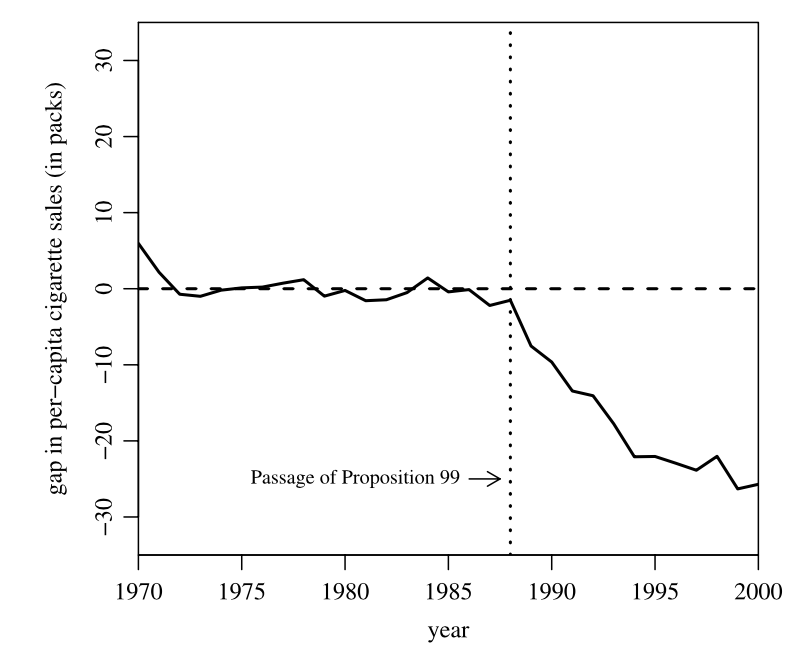
\includegraphics[height=0.66\textheight]{abadie_4.png}
\end{column}
\end{columns}
\medskip
Synthetic California is mostly Utah, Nevada, Montana, Colorado, and Connecticut. Left: real vs.\ synthetic sales. Right: the gap.
\end{frame}


\begin{frame}{Is California unusual? Placebo tests}
\begin{columns}
\begin{column}{0.55\textwidth}
\centering
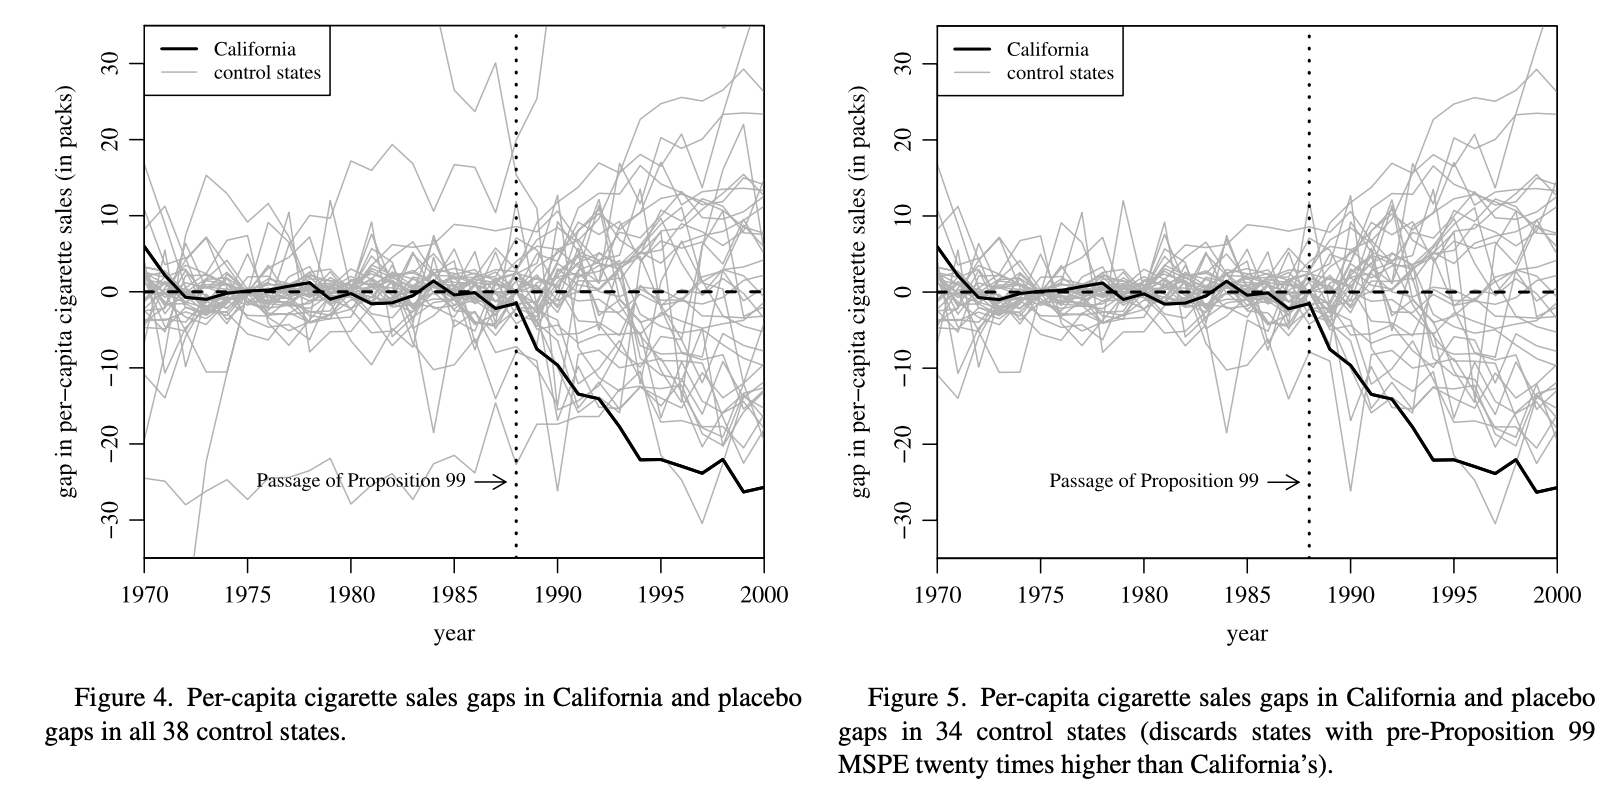
\includegraphics[width=\textwidth]{abadie_5.png}
\end{column}
\begin{column}{0.43\textwidth}
\begin{itemize}
	\item Pretend each other state passed Prop 99 in 1988 and build a synthetic control for it.
	\item If California's gap looks like the placebo gaps, we've learned nothing.
	\item Here California stands out. This comparison \alert{is} the inference.
\end{itemize}
\end{column}
\end{columns}
\end{frame}


\begin{frame}{DiD, synthetic control, or synthetic DiD?}
All three are \alert{weighted comparisons} of treated and control units before and after:
\begin{itemize}
	\item \alert{Many treated units, similar trends}: difference-in-differences.
	\item \alert{One or a few treated units} that a mix of controls can mimic: synthetic control.
	\item \alert{A treated unit whose level is unusual but whose trend is not}: synthetic DiD (Arkhangelsky et al.\ 2021). It weights controls to match the trend, then differences out the level gap.
	\item \alert{A treated unit with an extreme trend} (fastest-growing city, biggest firm): none of them works. Say so.
\end{itemize}
\medskip
R: \texttt{Synth}, \texttt{tidysynth}, \texttt{synthdid}.
\end{frame}


% =====================================================================
\section{Cutoffs: Regression Discontinuity}
% =====================================================================

\begin{frame}{Rules with cutoffs are everywhere}
Suppose Stern's honors program required a GPA of at least 3.5 to write a thesis.
\begin{itemize}
	\item Students at 3.49 and 3.51 are \alert{nearly identical}: same ability, same ambition, give or take a lucky grade.
	\item But only one of them can write a thesis.
	\item Compare outcomes \alert{just above} vs.\ \alert{just below} the cutoff: that is close to a lottery.
\end{itemize}
\medskip
This is \alert{regression discontinuity} (RD). The variable that determines treatment (GPA) is the \alert{running variable}.
\begin{itemize}
	\item Cutoffs show up in test-score admissions, vote shares, age limits, income eligibility, firm-size rules, ratings\ldots
\end{itemize}
\end{frame}


\begin{frame}{RD in a picture}
\centering
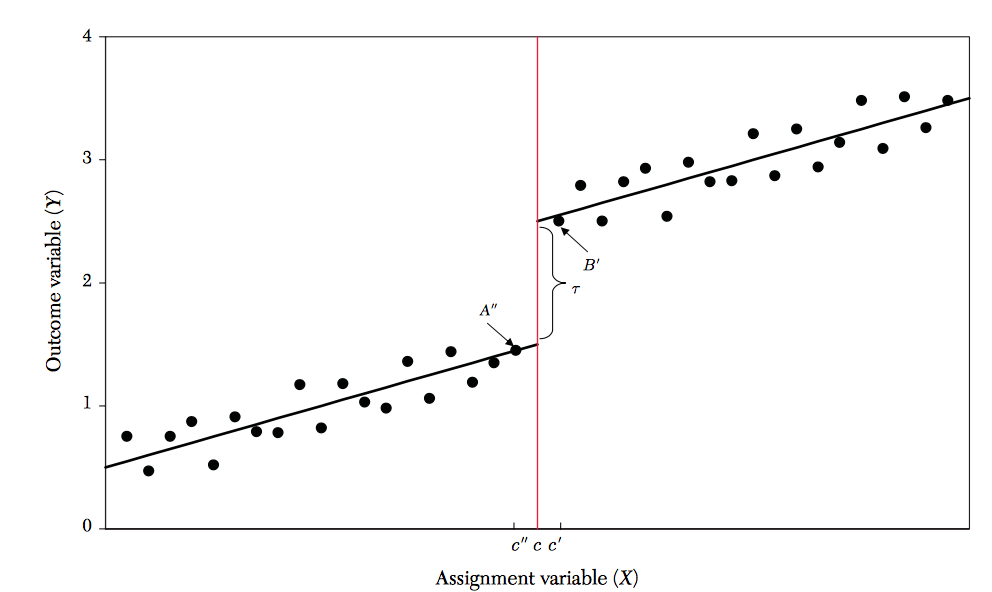
\includegraphics[height=0.85\textheight]{ll-fig1.png}
\end{frame}


\begin{frame}{What has to be true}
\begin{itemize}
	\item \alert{Nothing else jumps at the cutoff.} If 3.5 also triggers Latin honors or a recruiting list, you can't separate the thesis effect from those.
	\item \alert{People can't precisely sort around the cutoff.}
	\begin{itemize}
		\item If students can lobby professors for a grade bump to 3.5, the ones just above differ from the ones just below.
		\item Examples: under-reporting income to qualify for a program, drug quantities charged just below thresholds.
	\end{itemize}
	\item You learn the effect \alert{at the cutoff}. Effects for 3.0 or 3.9 students may differ.
	\item If crossing the cutoff only raises the \emph{chance} of treatment, you have a \alert{fuzzy RD}: it works like IV, and the cutoff is the instrument.
\end{itemize}
\end{frame}


\begin{frame}{Lee (2008): do incumbents have an advantage?}
\begin{itemize}
	\item Incumbents win re-election far more often. Does holding office help, or are good politicians just good?
	\item \alert{Running variable}: the Democrat's vote margin in the previous House election.
	\item Compare districts where Democrats \alert{barely won} to districts where they \alert{barely lost}.
	\item Barely winning vs.\ barely losing a close election is close to a coin flip.
\end{itemize}
\end{frame}


\begin{frame}{Lee (2008)}
\begin{columns}
\begin{column}{0.5\textwidth}
\centering
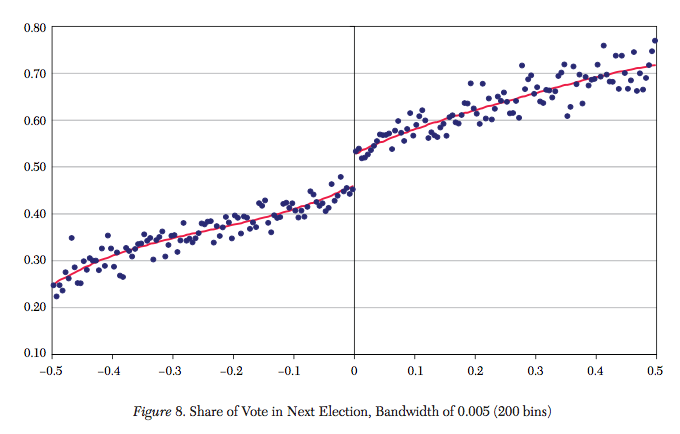
\includegraphics[width=\textwidth]{binscatter1.png}
\end{column}
\begin{column}{0.5\textwidth}
\centering
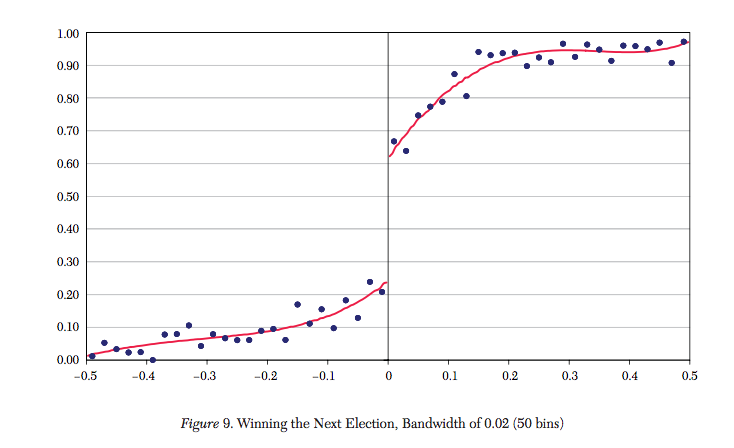
\includegraphics[width=\textwidth]{binscatter2.png}
\end{column}
\end{columns}
\medskip
\centering
Barely winning raises the chance of winning \alert{next time} by about 40 percentage points.
\end{frame}


\begin{frame}{Checking for sorting (McCrary 2008)}
\begin{columns}
\begin{column}{0.5\textwidth}
\centering
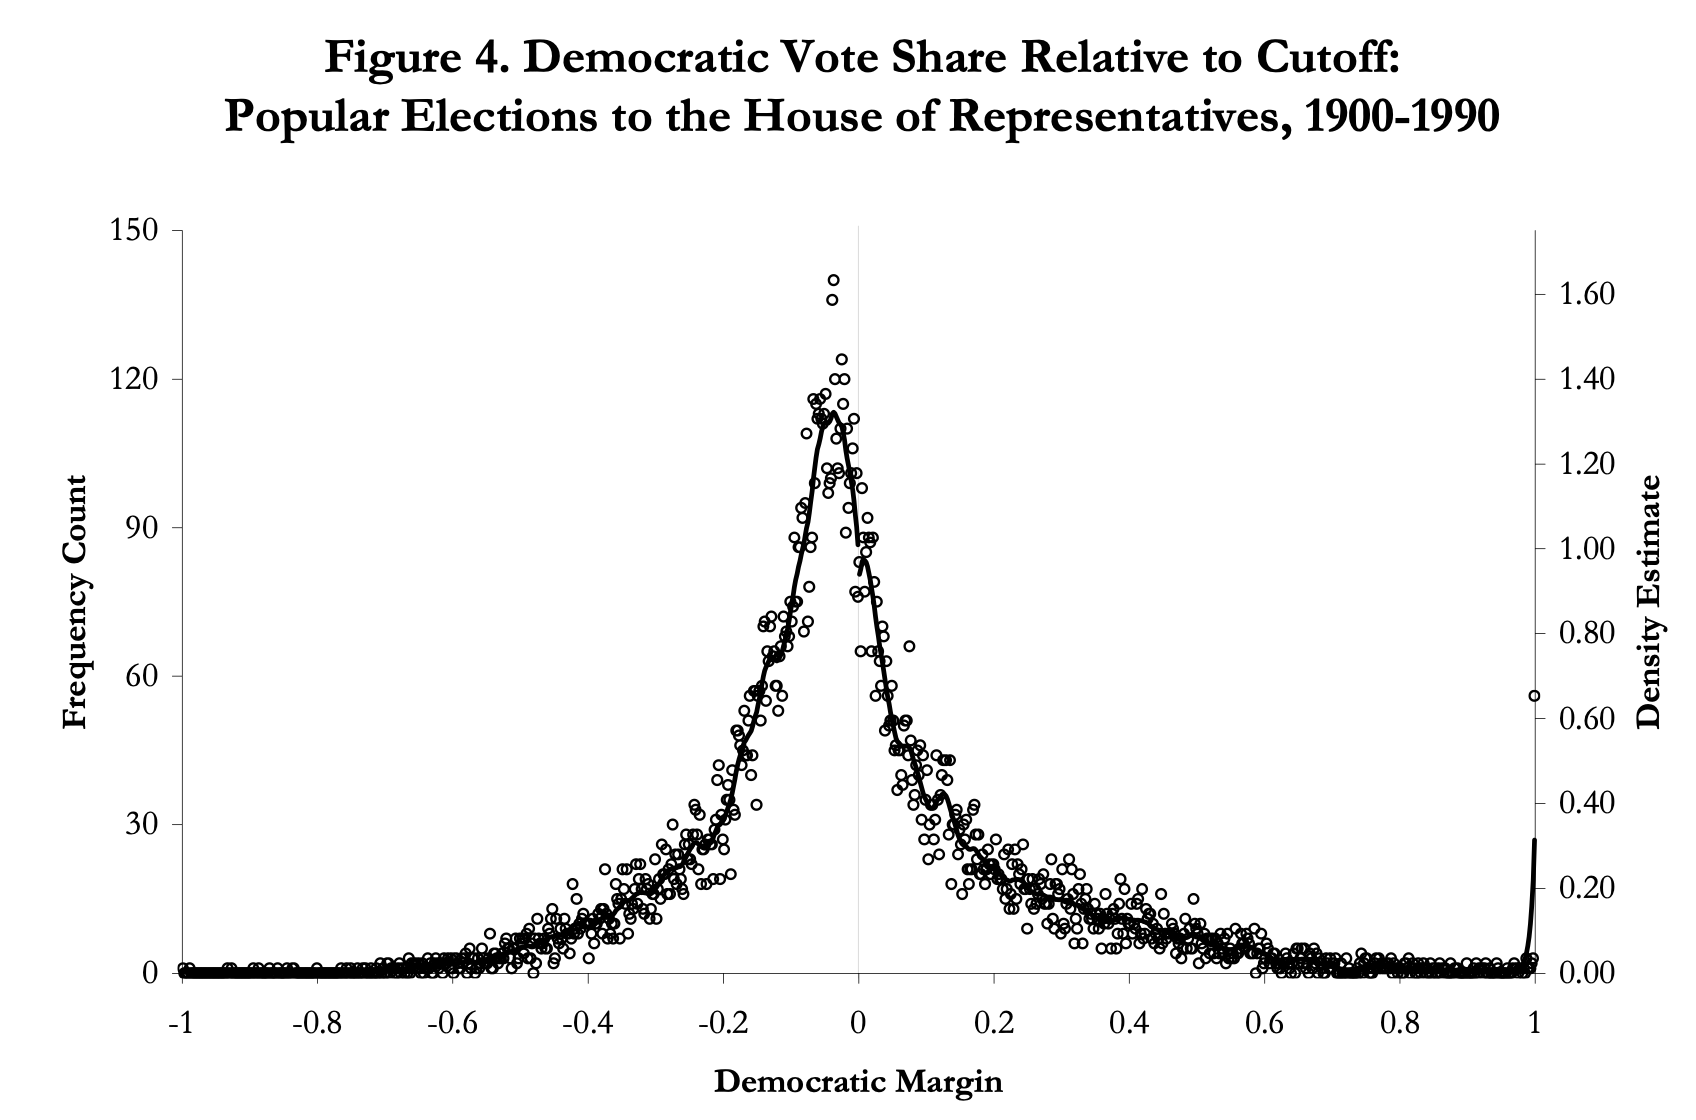
\includegraphics[height=0.62\textheight]{mccrary2.png}\\
{\small House elections: smooth density}
\end{column}
\begin{column}{0.5\textwidth}
\centering
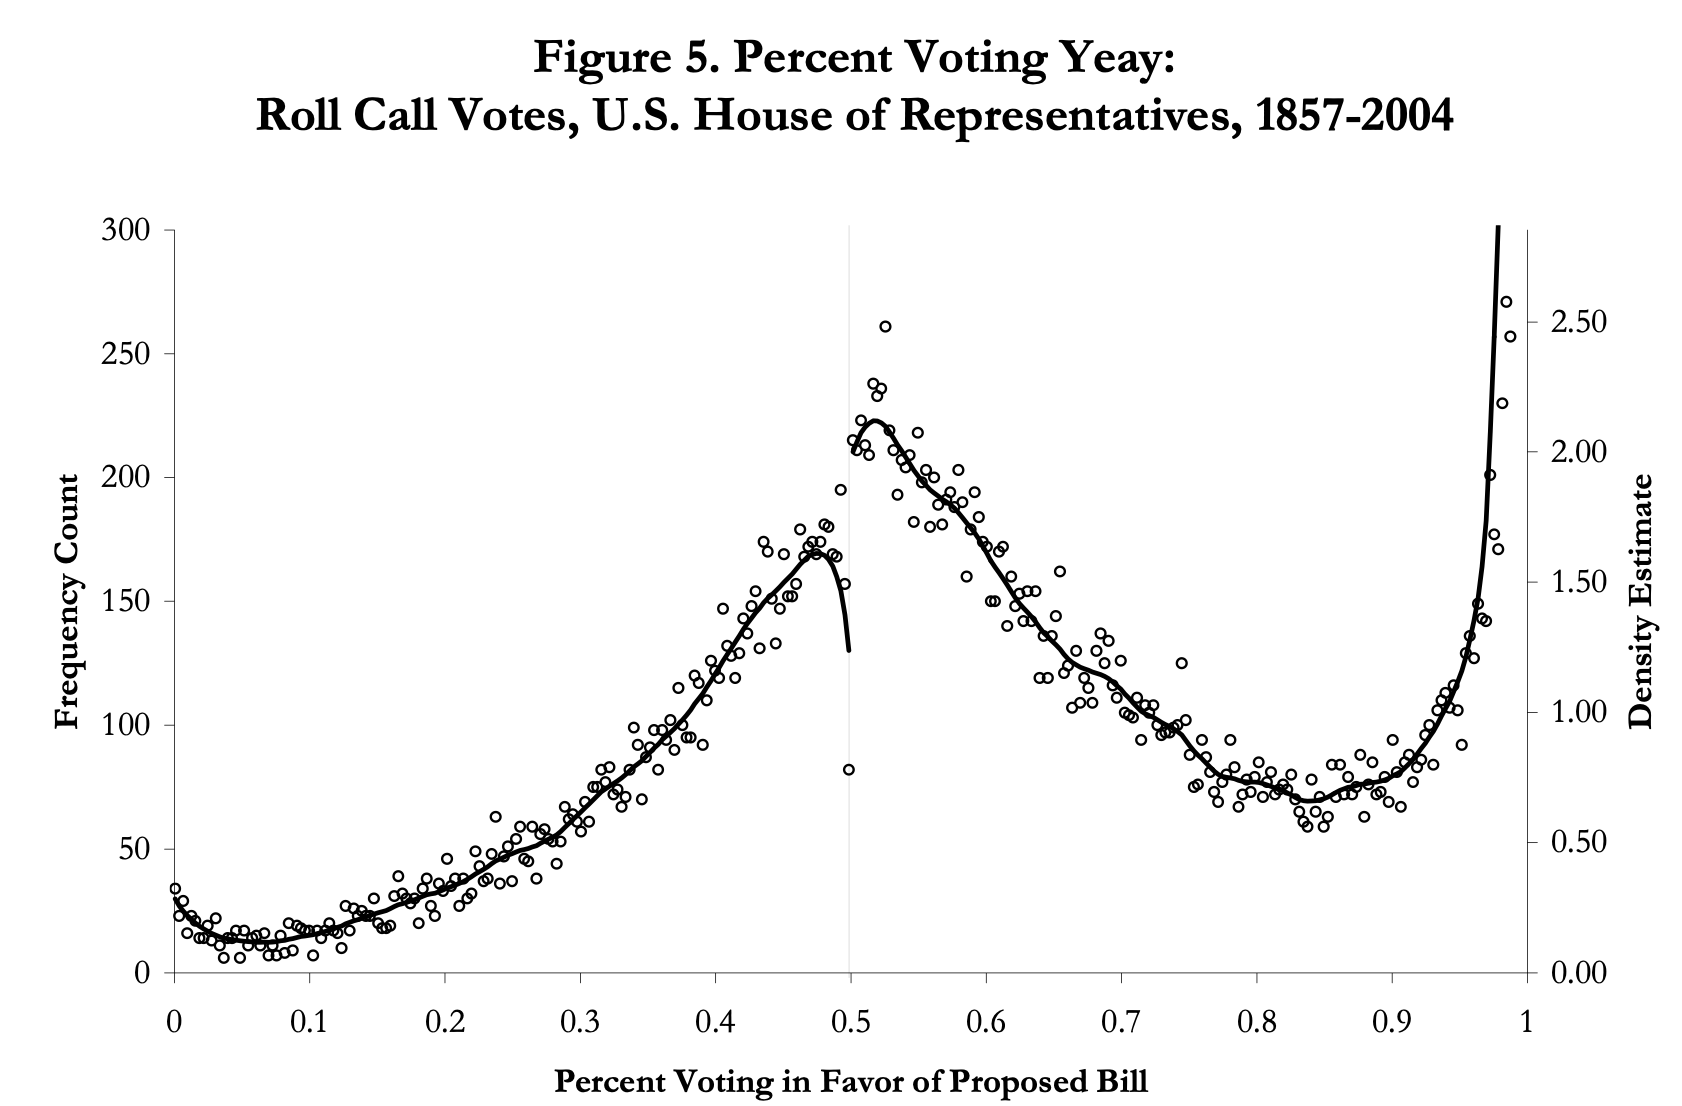
\includegraphics[height=0.62\textheight]{mccrary3.png}\\
{\small Roll-call votes: bunching just above 50\%}
\end{column}
\end{columns}
\medskip
If the number of units \alert{jumps} at the cutoff, people are sorting and the design is in trouble.
\end{frame}


\begin{frame}{What every RD paper shows}
\begin{enumerate}
	\item A plot of \alert{treatment} against the running variable: the jump in treatment.
	\item A plot of the \alert{outcome}: the jump you are claiming.
	\item Plots of \alert{pre-determined characteristics}: these should \emph{not} jump.
	\item The \alert{density} of the running variable: no bunching.
	\item Estimates using a \alert{local linear} fit near the cutoff, robust to the choice of bandwidth.
\end{enumerate}
\medskip
\begin{itemize}
	\item Avoid high-order polynomials fit to the whole range (Gelman \& Imbens 2019).
	\item Tools: \texttt{rdrobust}, \texttt{rddensity}, \texttt{rdplot} (Cattaneo, Idrobo \& Titiunik) in R, Stata, and Python.
\end{itemize}
\end{frame}


\begin{frame}{More cutoffs}
\begin{itemize}
	\item \alert{Yelp ratings} (Luca): a restaurant's average gets rounded to the nearest half-star. Compare 3.74 to 3.76 to measure the effect of an extra half star on revenue.
	\item \alert{Class size} (Angrist \& Lavy 1999): Israeli schools split classes when enrollment passes 40, so class size jumps at 41, 81, \ldots
	\item \alert{Elite exam schools} (Abdulkadiro\u{g}lu, Angrist \& Pathak 2014): students just above vs.\ just below the admission score in Boston and New York do about the same later. The ``elite'' effect is mostly selection.
\end{itemize}
\end{frame}


% =====================================================================
\section{Final Thoughts}
% =====================================================================

\begin{frame}{Always be asking}
\begin{itemize}
	\item What am I trying to \alert{measure}, and for \alert{whom}?
	\item What is my \alert{counterfactual}?
	\item Why do treated and untreated units differ? What is my \alert{selection problem}?
	\item What \alert{plausibly random} variation can I use?
	\item What must be true for my design to work, and \alert{what evidence can I show} for it?
	\item Am I controlling for something the treatment \alert{caused}, or choosing my sample on an outcome?
\end{itemize}
\medskip
Don't look for your keys only where the light is. But you could do a lot worse than following one of the scripts above.
\end{frame}


\begin{frame}{Where to read more}
\begin{itemize}
	\item Angrist \& Pischke, \alert{\emph{Mastering 'Metrics}}: the most readable introduction, written for undergraduates.
	\item Huntington-Klein, \alert{\emph{The Effect}} (\href{https://theeffectbook.net}{theeffectbook.net}): free, with code in R, Stata, and Python.
	\item Cunningham, \alert{\emph{Causal Inference: The Mixtape}} (\href{https://mixtape.scunning.com}{mixtape.scunning.com}): free, with code.
	\item Roth, Sant'Anna, Bilinski \& Poe (2023), ``What's Trending in Difference-in-Differences?'': a readable survey of the new DiD methods.
\end{itemize}
\end{frame}

\end{document}
